

\documentclass{ctexart}
\usepackage{amsmath,bm}
\usepackage{setspace}
\usepackage{xeCJK}
\usepackage{xcolor}
\usepackage{indentfirst}
\usepackage{listings}
\usepackage{graphicx}
\usepackage{subfigure}
\usepackage{amsfonts,amssymb}
\usepackage[a4paper,scale=0.8]{geometry}
\usepackage{hyperref}
\usepackage{float}
\usepackage{listings}
\usepackage{changepage}
\usepackage{longtable}

\usepackage{float}
\definecolor{gray}{rgb}{0.5,0.5,0.5}
\definecolor{dkgreen}{rgb}{.068,.578,.068}
\definecolor{dkpurple}{rgb}{.320,.064,.680}

% set Matlab styles
\lstset{
   language=Matlab,
   numbers=left,
   keywords={break,case,catch,continue,else,elseif,end,for,function,
      global,if,otherwise,persistent,return,switch,try,while},
   basicstyle=\ttfamily,
   keywordstyle=\color{blue}\bfseries,
   commentstyle=\color{dkgreen},
   stringstyle=\color{dkpurple},
   backgroundcolor=\color{white},
   breaklines=true,
   tabsize=4,
   showspaces=false,
   showstringspaces=false,
}
\setCJKmainfont{华光书宋_CNKI}
\newCJKfontfamily\kaiti{华光楷体_CNKI}
\newCJKfontfamily\hei{华光黑体_CNKI}
\newCJKfontfamily\fsong{华光仿宋_CNKI}
\newfontfamily\code{Courier New}
\linespread{1.5} \setlength\parindent{2 em}
\title{\Huge 中国科学技术大学计算机学院\\《数字图像处理与分析》实验报告}
\date{\LARGE 2021.06.15}
\begin{document}
\begin{hei}  \maketitle\end{hei}
\begin{figure}[htbp]
    \centering
    
\includegraphics[scale=0.4]{USTC.png}

\end{figure}
\begin{LARGE}\begin{align*}      & \text{实验题目:\underline{图像处理实验}} \\
         & \text{学生姓名:\underline{胡毅翔}}       \\
         & \text{学生学号:\underline{PB18000290}}\end{align*}\end{LARGE}
\par
\par\par
\centerline{\large 计算机实验教学中心制}
\par \centerline {\large 2019年9月}
\newpage
\tableofcontents
\newpage
\section{\hei 实验目的}
本实验的目的是通过实验进一步理解和掌握数字图像处理与分析的原理和方
法。通过分析、实现现有的图像处理算法,学习和掌握常用的图像处理与分析技术。

\section{\hei 实验环境}
\begin{enumerate}
    \item PC一台
    \item Windows 10操作系统
    \item Matlba 9.5.0.1033004 (R2018b) Update 2
    \item Visual Studio Code 1.56.2
\end{enumerate}
\section{\hei 实验内容}
数字图像处理的实验内容主要包括五个方面:
\begin{enumerate}
    \item 图像几何变换。
    \item 对图像进行空间域滤波,提高图像视觉质量, 以便于人眼观察、理解或用计算机对其进一步处
          理。
    \item 对图像作频域变换, 进行频率域滤波增强处理。
    \item 在空间域和频域提取、
          描述和分析图像中所包含的特征,便于计算机对图像作进一步的分析和理解, 经常作为模
          式识别和计算机视觉的预处理。这些特征包括很多方面,如图像的频域特性、边界特征
          等。
    \item 了解常见的图像退化模型和相应的图像恢复算法,从本质上改善图像质量;对
          图像进行分析,采用阈值法、区域分裂合并法等分割算法,获取图像中感兴趣目标区域。
\end{enumerate}
\section{\hei 实验一\ 图像几何变换}
\subsection{\hei 图像的平移}
\subsubsection{\hei 实验原理}
图像平移就是将图像中所有的点都按照指定的平移量水平、垂直移动。如:设 $\left(x_{0}, y_{0}\right)$ 为原图像的一点,图像水平平移量为 tx,垂直平移量为 ty,则平移后坐标变为
$\left(x_{1}, y_{1}\right)$, 显然, $\left(x_{0}, y_{0}\right)$ 和 $\left(x_{1}, y_{1}\right)$ 有如下关系:
$$\left\{\begin{array}{l}x_{1}=x_{0}+t x \\ y_{1}=y_{0}+t y\end{array}\right.$$
用矩阵表示如下:
$$\left[\begin{array}{l}x_{1} \\ y_{1} \\ 1\end{array}\right]=\left[\begin{array}{lll}1 & 0 & \mathrm{tx} \\ 0 & 1 & \mathrm{ty} \\ 0 & 0 & 1\end{array}\right]\left[\begin{array}{l}x_{0} \\ y_{0} \\ 1\end{array}\right]$$
\subsubsection{\hei 实验内容}
输入一幅图像,根据输入的水平和垂直平移量,显示平移后的图像。
\par 输入水平偏移量$100$,垂直偏移量$100$,得到的结果为:
\begin{figure}[H]
    \centering
    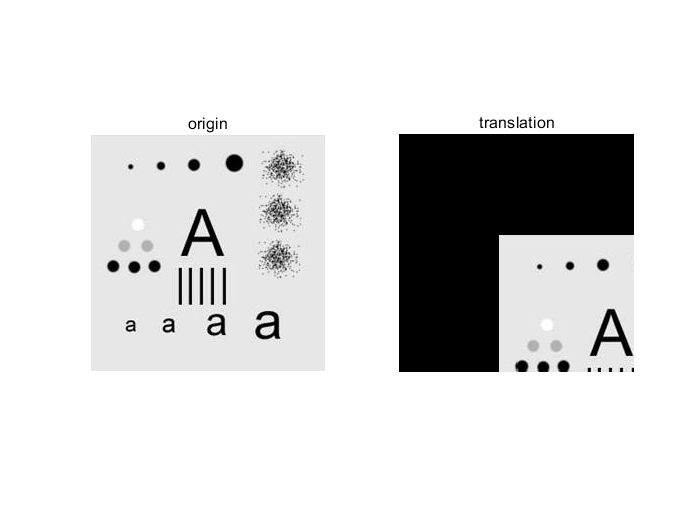
\includegraphics[scale=0.5]{1_1.png}
    \caption{图像的平移}
\end{figure}

\subsection{\hei 图像的旋转}
\subsubsection{\hei 实验原理}
图像绕中心点(原点)旋转的公式如下:
$\left[\begin{array}{l}x_{1} \\ y_{1} \\ 1\end{array}\right]=\left[\begin{array}{lll}\cos (\theta) & -\sin (\theta) & 0 \\ \sin (\theta) & \cos (\theta) & 0 \\ 0 & 0 & 1\end{array}\right]\left[\begin{array}{l}x_{0} \\ y_{0} \\ 1\end{array}\right]$
图像如果绕一个指定点 $(a, b)$ 旋转,则先要将坐标系平移到该点,再进行旋转,然后 平移回新的坐标原点。则旋转变换表达式为:
$$\left[\begin{array}{l}x_{1} \\ y_{1} \\ 1\end{array}\right]=\left[\begin{array}{ccc}1 & 0 & \mathrm{a} \\ 0 & 1 & \mathrm{~b} \\ 0 & 0 & 1\end{array}\right]\left[\begin{array}{lcc}\cos (\theta) & -\sin (\theta) & 0 \\ \sin (\theta) & \cos (\theta) & 0 \\ 0 & 0 & 1\end{array}\right]\left[\begin{array}{ccc}1 & 0 & -\mathrm{a} \\ 0 & 1 & -\mathrm{b} \\ 0 & 0 & 1\end{array}\right]\left[\begin{array}{l}\boldsymbol{x}_{0} \\ y_{0} \\ 1\end{array}\right]$$
\subsubsection{\hei 实验内容}
输入一幅图像,根据输入的旋转角度参数,绕图像中心点旋转,分别用最近邻
插值和双线性插值显示旋转后的图像。
\par 输入旋转角度参数$60$,得到的结果为:
\begin{figure}[H]
    \centering
    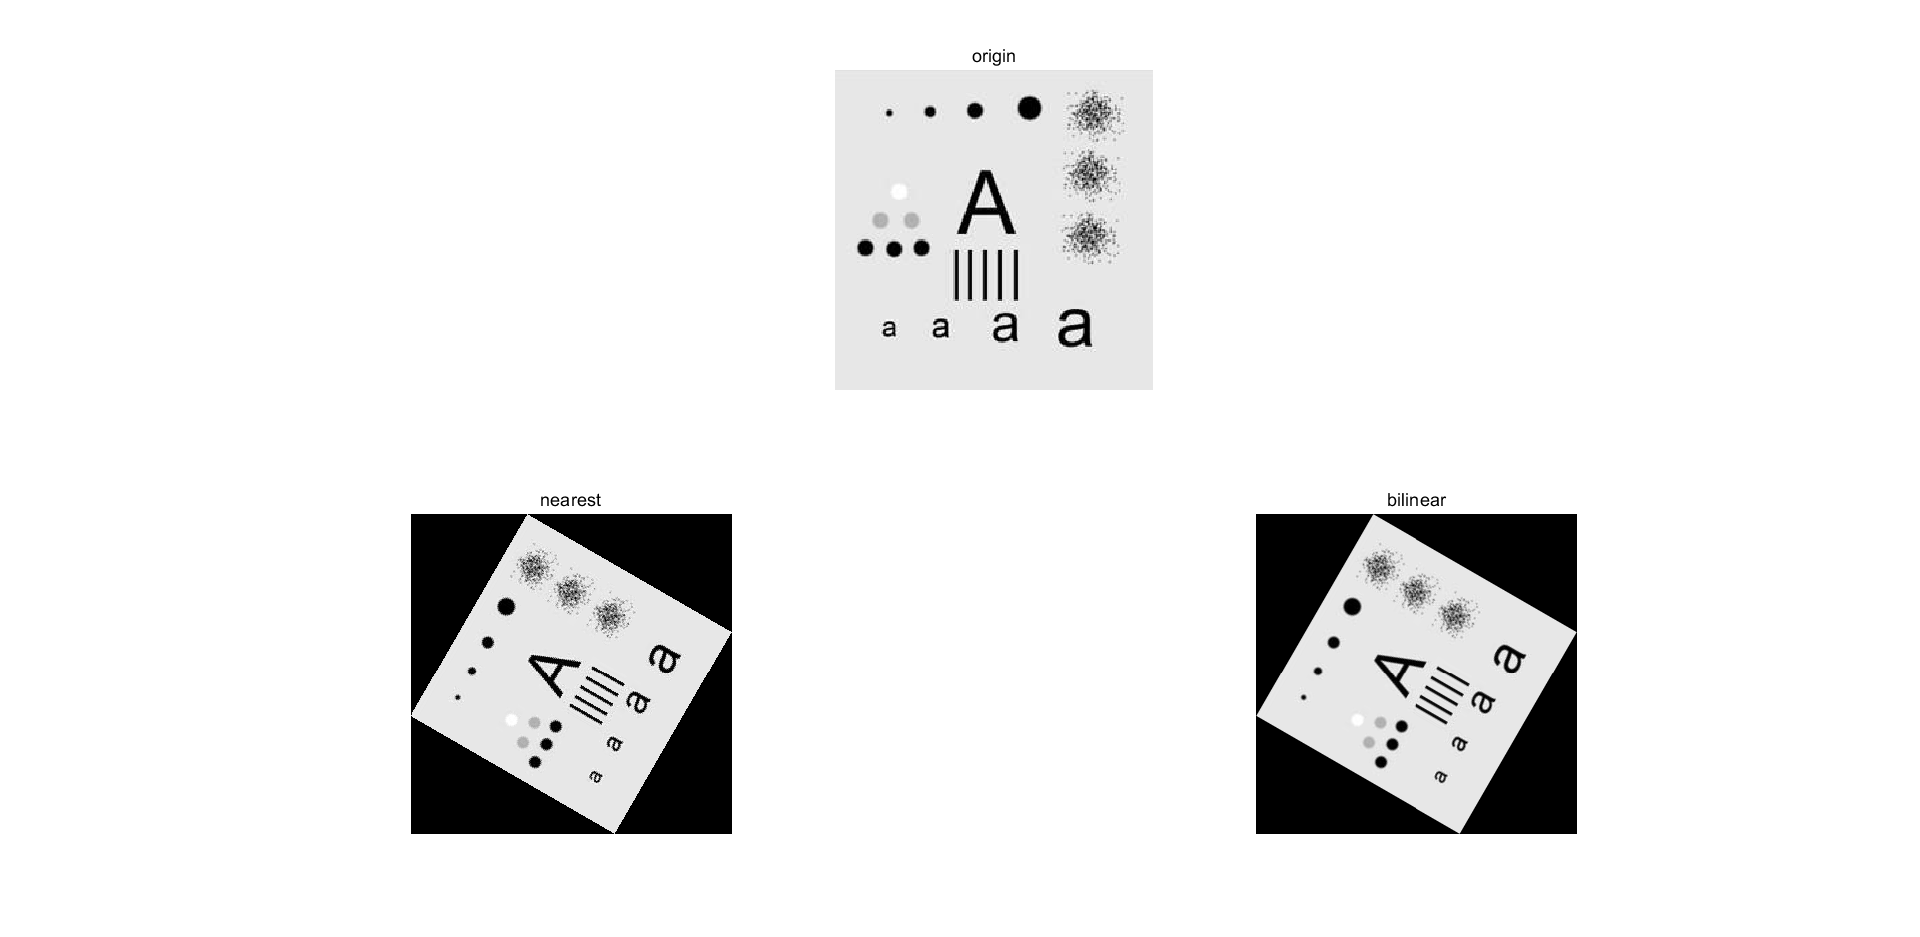
\includegraphics[scale=0.3]{1_2.png}
    \caption{图像的旋转}
\end{figure}
\subsection{\hei 图像的缩放}
\subsubsection{\hei 实验原理}
假设图像 $\mathrm{x}$ 轴方向缩放比率为 $\mathrm{c}, \mathrm{y}$ 轴方向缩放比率为 $\mathrm{d}$, 那么原图中,点 $\left(x_{0}, y_{0}\right)$ 对应 于新图中的点 $\left(x_{1}, y_{1}\right)$ 的转换矩阵为:
$$
    \left[\begin{array}{l}
            x_{1} \\
            y_{1} \\
            1
        \end{array}\right]=\left[\begin{array}{lll}
            c & 0           & 0 \\
            0 & \mathrm{~d} & 0 \\
            0 & 0           & 1
        \end{array}\right]\left[\begin{array}{l}
            \boldsymbol{x}_{0} \\
            y_{0}              \\
            1
        \end{array}\right]
$$
\subsubsection{\hei 实验内容}
输入一幅图像,根据输入的水平和垂直缩放量,分别用最近邻插值和双线性插值,
显示缩放后的图像。
\par 水平方向缩放为原来的$1/3$,垂直方向缩放为原来的$1/2$,得到的结果为:
\begin{figure}[H]
    \centering
    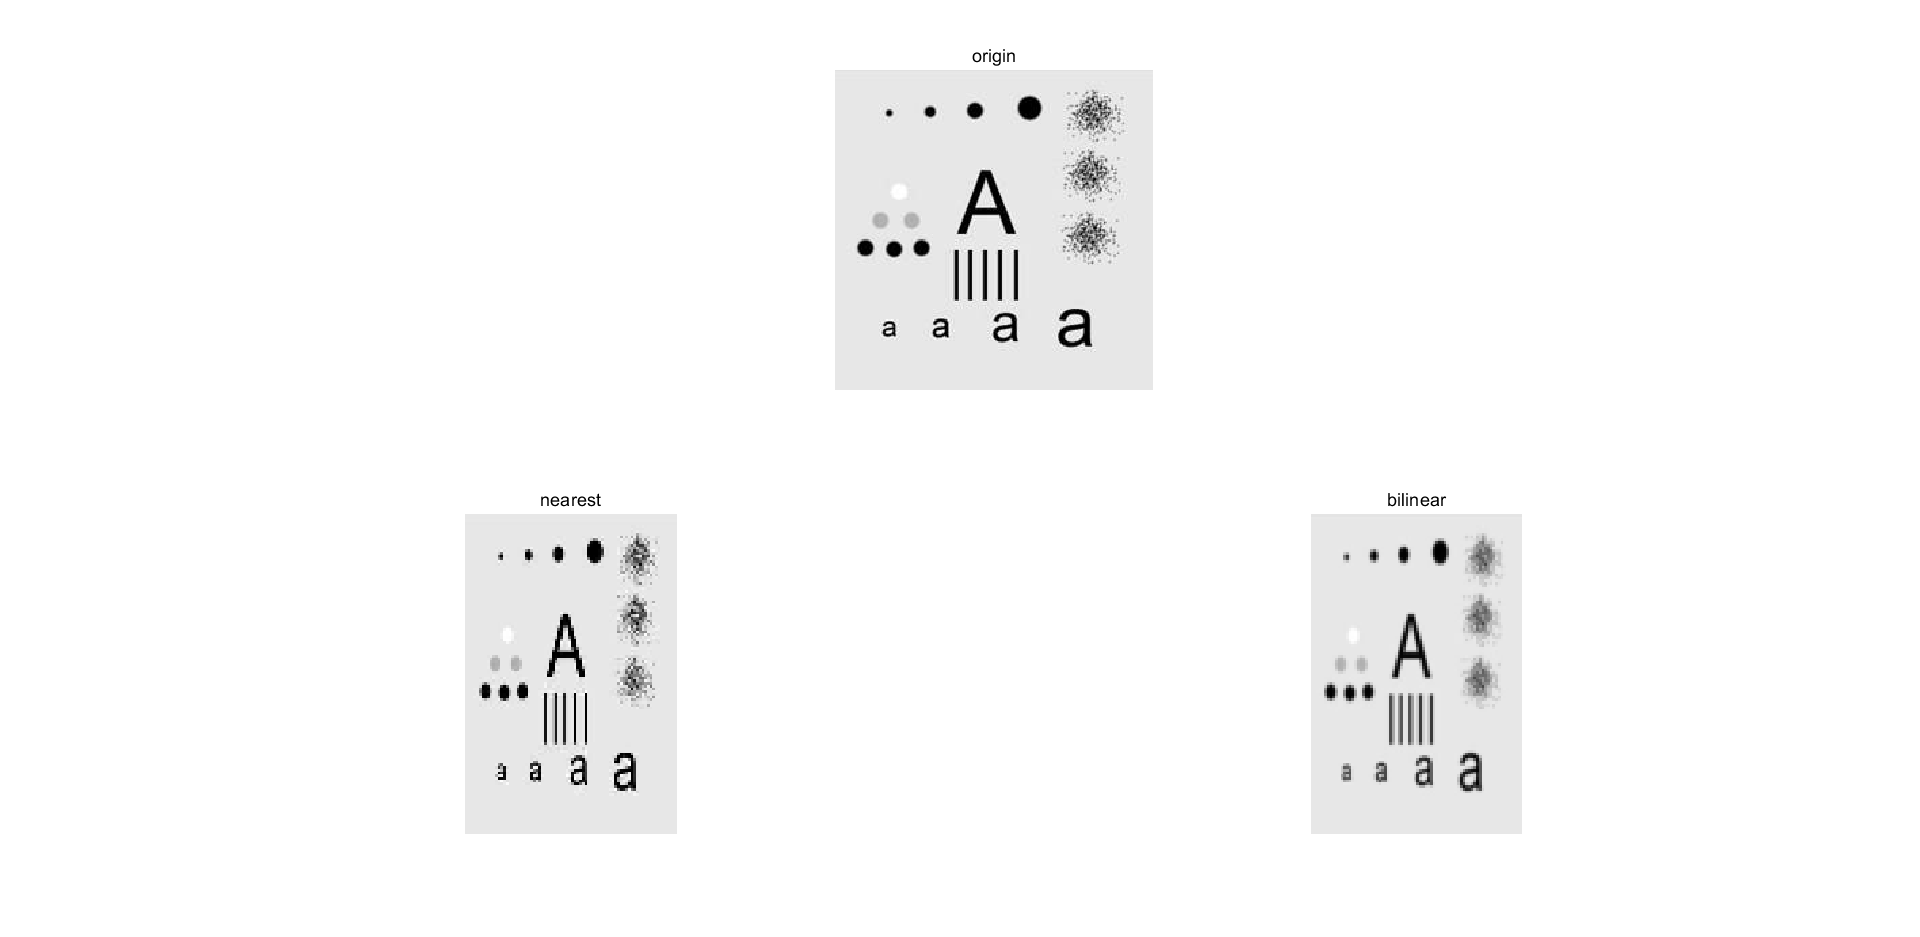
\includegraphics[scale=0.3]{1_3.png}
    \caption{图像的缩放}
\end{figure}
\subsection{\hei 图像几何失真校正}
\subsubsection{\hei 实验原理}
设原图像: $\mathrm{f}(\mathrm{x}, \mathrm{y}) \quad$ 失真图像:g $\left(\mathrm{x}^{\prime}, \mathrm{y}^{\prime}\right)$
$$\mathrm{x}^{\prime}=\mathrm{s}(\mathrm{x}, \mathrm{y})$$
$$\mathrm{y}^{\prime}=\mathrm{t}(\mathrm{x}, \mathrm{y})$$
通过选取控制点对, 求出 $\left(\mathrm{x}^{\prime}, \mathrm{y}^{\prime}\right)$ 与 $(\mathrm{x}, \mathrm{y})$ 坐标之间的关系
\begin{enumerate}\item  线性失真: $$\mathrm{x}^{\prime}=\mathrm{a}_{1} \mathrm{x}+\mathrm{a}_{2} \mathrm{y}+\mathrm{a}_{3}$$
          $$\mathrm{y}^{\prime}=\mathrm{b}_{1} \mathrm{x}+\mathrm{b}_{2} \mathrm{y}+\mathrm{b}_{3}$$
          6个系数要3个控制点对 为减少误差, 选取n>3个控制点对
          $$\left[\begin{array}{c}x_{1}^{\prime} \\ x_{2}^{\prime} \\ . \\ . \\ \vdots \\ x_{n}^{\prime}\end{array}\right]=\left[\begin{array}{rrr}x_{1} & y_{1} & 1 \\ x_{2} & y_{2} & 1 \\ \cdot & \cdot & \cdot \\ \cdot & \cdot & \cdot \\ \cdot & \cdot & \cdot \\ x_{n} & y_{n} & 1\end{array}\right]\left[\begin{array}{l}a_{1} \\ a_{2} \\ a_{3}\end{array}\right]$$
          $$\mathrm{M}=\left[\begin{array}{ccc}x_{1} & y_{1} & 1 \\ x_{2} & y_{2} & 1 \\ \cdot & \cdot
                                 & \cdot     \\ \cdot & \cdot & \cdot \\ \cdot & \cdot & \cdot \\ x_{n} & y_{n} & 1\end{array}
                  \right]\left[\begin{array}{l}a_{1} \\ a_{2} \\ a_{3}\end{array}\right]=\left(\mathrm{M}^{\mathrm{T}}
              \mathrm{M}\right)^{-1} \mathrm{M}^{\mathrm{T}}\left[\begin{array}{c}x_{1}^{\prime} \\ x_{2}^{\prime}
                      \\ \cdot \\ \cdot \\ \vdots \\ x_{n}^{\prime}\end{array}\right] \quad\left[\begin{array}{l}b_{1}
                      \\ b_{2} \\ b_{3}\end{array}\right]=\left(\mathrm{M}^{\mathrm{T}} \mathrm{M}\right)^{-1}
              \mathrm{M}^{\mathrm{T}}\left[\begin{array}{c}y_{1}^{\prime} \\ y_{2}^{\prime} \\ \cdot \\ \cdot \\
                      y_{n}^{\prime}\end{array}\right]$$
    \item 双线性失真:$$\left\{\begin{array}{l}x^{\prime}=a_{1} x y+a_{2} x+a_{3} y+a_{4} \\ y^{\prime}=b_{1} x y+b_{2} x+b_{3} y+b_{4}\end{array}\right.$$
          8个系数要4个控制点对 为减少误差, 选取n>4个控制点对
          $$\mathrm{M}=\left[\begin{array}{cccc}x_{1} y_{1} & x_{1} & y_{1} & 1
                      \\ x_{2} y_{2} & x_{2} & y_{2} & 1 \\ \cdot & \cdot & \cdot & \cdot \\ \cdot & \cdot & \cdot & \cdot
                      \\ \cdot & \cdot & \cdot & \cdot \\ x_{n} y_{n} & x_{n} & y_{n} &
                      1\end{array}\right]\left[\begin{array}{c}a_{1} \\ a_{2} \\ a_{3} \\ a_{4}\end{array}\right]=\left(\mathrm{M}^{\mathrm{T}}
              \mathrm{M}\right)^{-1} \mathrm{M}^{\mathrm{T}}\left[\begin{array}{c}x_{1}^{\prime} \\ x_{2}^{\prime} \\ \cdot \\ \cdot \\ \vdots_{n}^{\prime}\end{array}\right]\left[\begin{array}{c}b_{1} \\ b_{2} \\ b_{3} \\ b_{4}\end{array}\right]=\left(\mathrm{M}^{\mathrm{T}} \mathrm{M}\right)^{-1} \mathrm{M}^{\mathrm{T}}
              \left[\begin{array}{c}y_{1}^{\prime} \\ y_{2}^{\prime} \\ \cdot \\ \cdot \\ y_{n}^{\prime}\end{array}\right]$$
    \item 二次校正式:

          $$x^{\prime}=a_{1} x^{2}+a_{2} y^{2}+a_{3} x y+a_{4} x+a_{5} y+a_{6}$$
          $$y^{\prime}=b_{1} x^{2}+b_{2} y^{2}+b_{3} x y+b_{4} x+b_{5} y+b_{6}$$
          12个系数要6个控制点对 为减少误差, 选取n>6个控制点对
          $$
              \begin{aligned}
                  &{\left[\begin{array}{l}
                          a_{1} \\
                          a_{2} \\
                          a_{3} \\
                          a_{4} \\
                          a_{5} \\
                          a_{6}
                      \end{array}\right]=\left(\mathrm{M}^{\mathrm{T}} \mathrm{M}\right)^{-1} \mathrm{M}^{\mathrm{T}}\left[\begin{array}{c}
                          x_{1}^{\prime} \\
                          x_{2}^{\prime} \\
                          \cdot          \\
                          \cdot          \\
                          \dot{x}_{n}^{\prime}
                      \end{array}\right]} \end{aligned}
          $$
          $$
              \begin{aligned}
                   & {\left[\begin{array}{c}
                          b_{1} \\
                          b_{2} \\
                          b_{3} \\
                          b_{4} \\
                          b_{5} \\
                          b_{6}
                      \end{array}\right]=\left(
                  \mathrm{M}^{\mathrm{T}} \mathrm{M}\right)^{-1}\mathrm{M}^{\mathrm{T}} \left[ \begin{array}{l} y_{1}^{\prime} \\
                          y_{2}^{\prime}     \\
                          \cdot              \\
                          \cdot              \\
                          y_{n}^{\prime}
                      \end{array}\right]}
              \end{aligned}
          $$
          $$\mathrm{M}=\left[\begin{array}{cccccc}x_{1}{ }^{2} & y_{1}{ }^{2} & x_{1} y_{1} & x_{1} & y_{1} & 1 \\ x_{2}{ }^{2} & y_{2}{ }^{2} & x_{2} y_{2} & x_{2} & y_{2} & 1 \\ \cdot & \cdot & \cdot & \cdot & \cdot & \cdot \\ \cdot & \cdot & \cdot & \cdot & \cdot & \cdot \\ \cdot & \cdot & \cdot & \cdot & \cdot & \cdot \\ x_{n}{ }^{2} & y_{n}{ }^{2} & x_{n} y_{n} & x_{n} & y_{n} & 1\end{array}\right]$$
\end{enumerate}
\subsubsection{\hei 实验内容}
输入图像 alphabet1.jpg 及几何失真图像 alphabet2.jpg,设置控制点进行几何失
真校正,显示校正后的图像。
\par 选取4个控制点:
\begin{figure}[H]
    \centering
    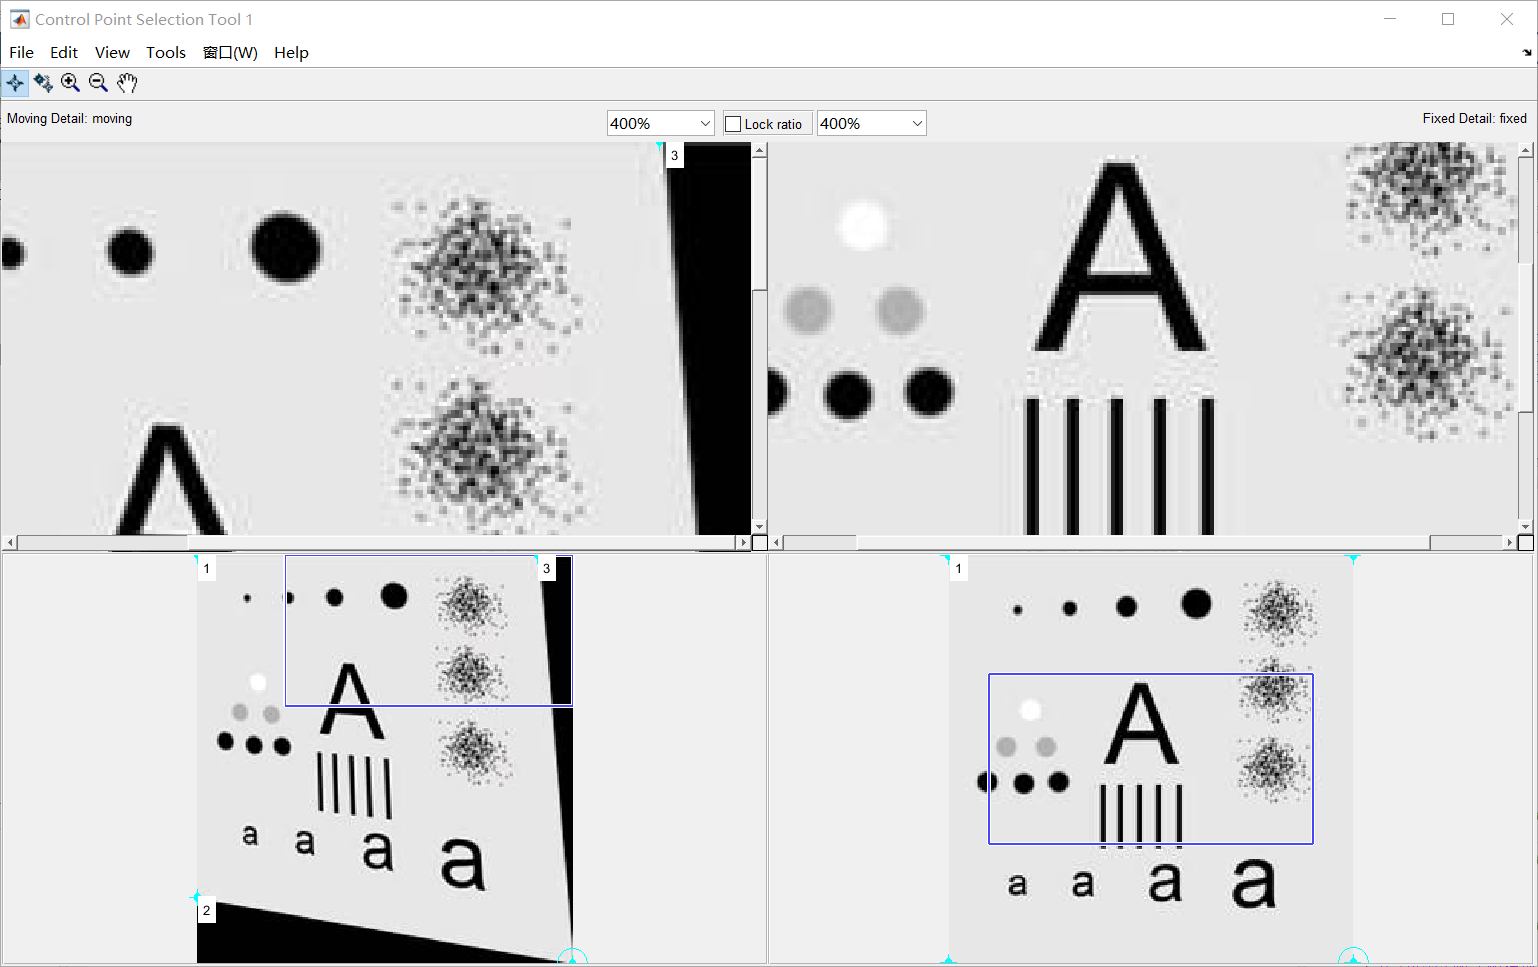
\includegraphics[scale=0.15]{1_4_1.png}
    \caption{控制点的选取}
\end{figure}
\par 得到的校正结果:
\begin{figure}[H]
    \centering
    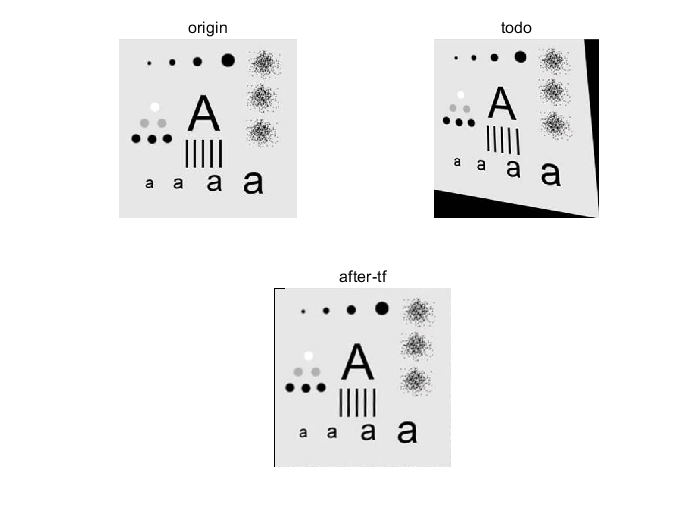
\includegraphics[scale=0.3]{1_4_2.png}
    \caption{图像几何失真校正}
\end{figure}
\section{\hei 实验二\ 图像点处理增强}
\subsection{\hei 灰度的线性变换}
\subsubsection{\hei 实验原理}
灰度的线性变换就是将图像中所有的点的灰度按照线性灰度变换函数进行变换。该线 性灰度变换函数是一个一维线性函数:
$$
    f(x)=f_{A} \cdot x+f_{B}
$$
灰度变换方程为:
$$D_{B}=f\left(D_{A}\right)=f_{A} \cdot D_{A}+f_{B}$$
其中参数 $f_{A}$ 为线性函数的斜率, $f_{B}$ 为线性函数的在 y 轴的截距, $D_{A}$ 表示输入图像的 灰度, $D_{B}$ 表示输出图像的灰度。
\subsubsection{\hei 实验内容}
输入一幅图像,根据输入的斜率和截距进行线性变换,并显示。
\par 关键函数为:
\begin{lstlisting}[frame=single]
function [new] = LinearTransformFunc(original, k, d)
    new = original;
    [a, b] = size(original);

    for i = 1:a

        for j = 1:b
            tmp = original(i, j) * k + d;

            if tmp > 255
                tmp = 255;
            elseif tmp < 0
                tmp = 0;
            end

            new(i, j) = tmp;
        end

    end

end
\end{lstlisting}
\par 输入的斜率为$3$,截距为$-44$,结果为:
\begin{figure}[H]
    \centering
    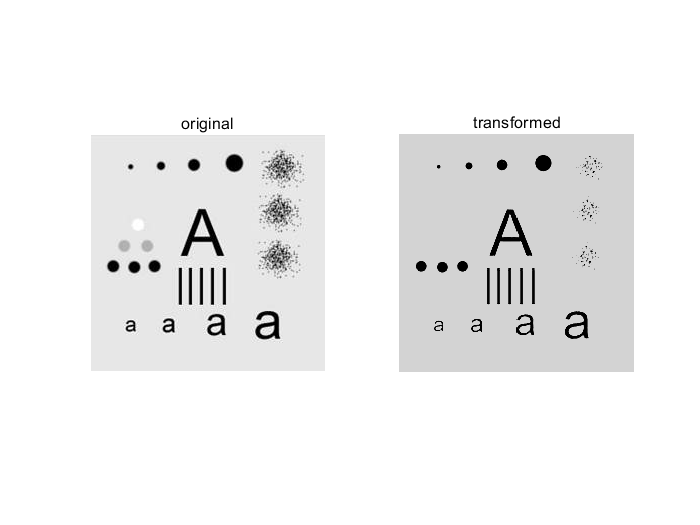
\includegraphics[scale=0.4]{2_1.png}
    \caption{灰度的线性变换}
\end{figure}

\subsection{\hei 灰度拉伸}
\subsubsection{\hei 实验原理}
灰度拉伸和灰度线性变换相似。不同之处在于它是分段线性变换。表达式如下:
$$f(x)=\frac{y_{1}}{x_{1}} x ; \quad x<x_{1}$$
$$f(x)=\frac{y_{2}-y_{1}}{x_{2}-x_{1}}\left(x-x_{1}\right)+y_{1} ; \quad x_{1} \leq x \leq x_{2}$$
$$f(x)=\frac{255-y_{2}}{255-x_{2}}\left(x-x_{2}\right)+y_{2} ; \quad x>x_{2}$$
其中, $\left(x_{1}, y_{1}\right)$ 和 $\left(x_{2}, y_{2}\right)$ 是分段函数的转折点。
\subsubsection{\hei 实验内容}
输入一幅图像,根据选择的转折点,进行灰度拉伸,显示变换后的图像。
\par 关键函数为:
\begin{lstlisting}[frame=single]
function [new] = StretchFunc(original, x1, y1, x2, y2)
    new = original;

    w = size(new, 1);
    h = size(new, 2);

    k1 = y1 / x1;

    dk1 = (y2 - y1) / (x2 - x1);
    dk2 = (255 - y2) / (255 - x2);

    for i = 1:w

        for j = 1:h
            x = new(i, j);

            if x < x1
                new(i, j) = k1 * x;
            elseif x < x2
                new(i, j) = dk1 * (x - x1) + y1;
            else
                new(i, j) = dk2 * (x - x2) + y2;
            end

            if new(i, j) > 255
                new(i, j) = 255;
            elseif new(i, j) < 0
                new(i, j) = 0;
            end

        end

    end

end
\end{lstlisting}
\par 参数$x_{1}, y_{1}, x_{2}, y_{2}$分别为
$30, 10, 200, 250$,得到的结果为:
\begin{figure}[H]
    \centering
    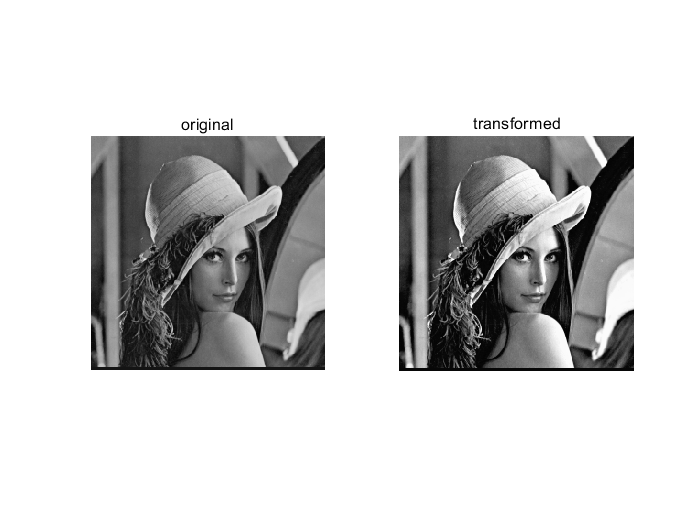
\includegraphics[scale=0.4]{2_2.png}
    \caption{灰度拉伸}
\end{figure}
\subsection{\hei 灰度直方图}
\subsubsection{\hei 实验原理}
灰度直方图是灰度值的函数,描述的是图像中具有该灰度值的像素的个数,其横坐标
表示像素的灰度级别,纵坐标表示该灰度出现的频率(象素的个数)。

\subsubsection{\hei 实验内容}
输入一幅图像,显示它的灰度直方图,可以根据输入的参数(上限、下限)显示特
定范围的灰度直方图。
\par 参数上限、下限分别为
$100, 255$,得到的结果为:
\begin{figure}[H]
    \centering
    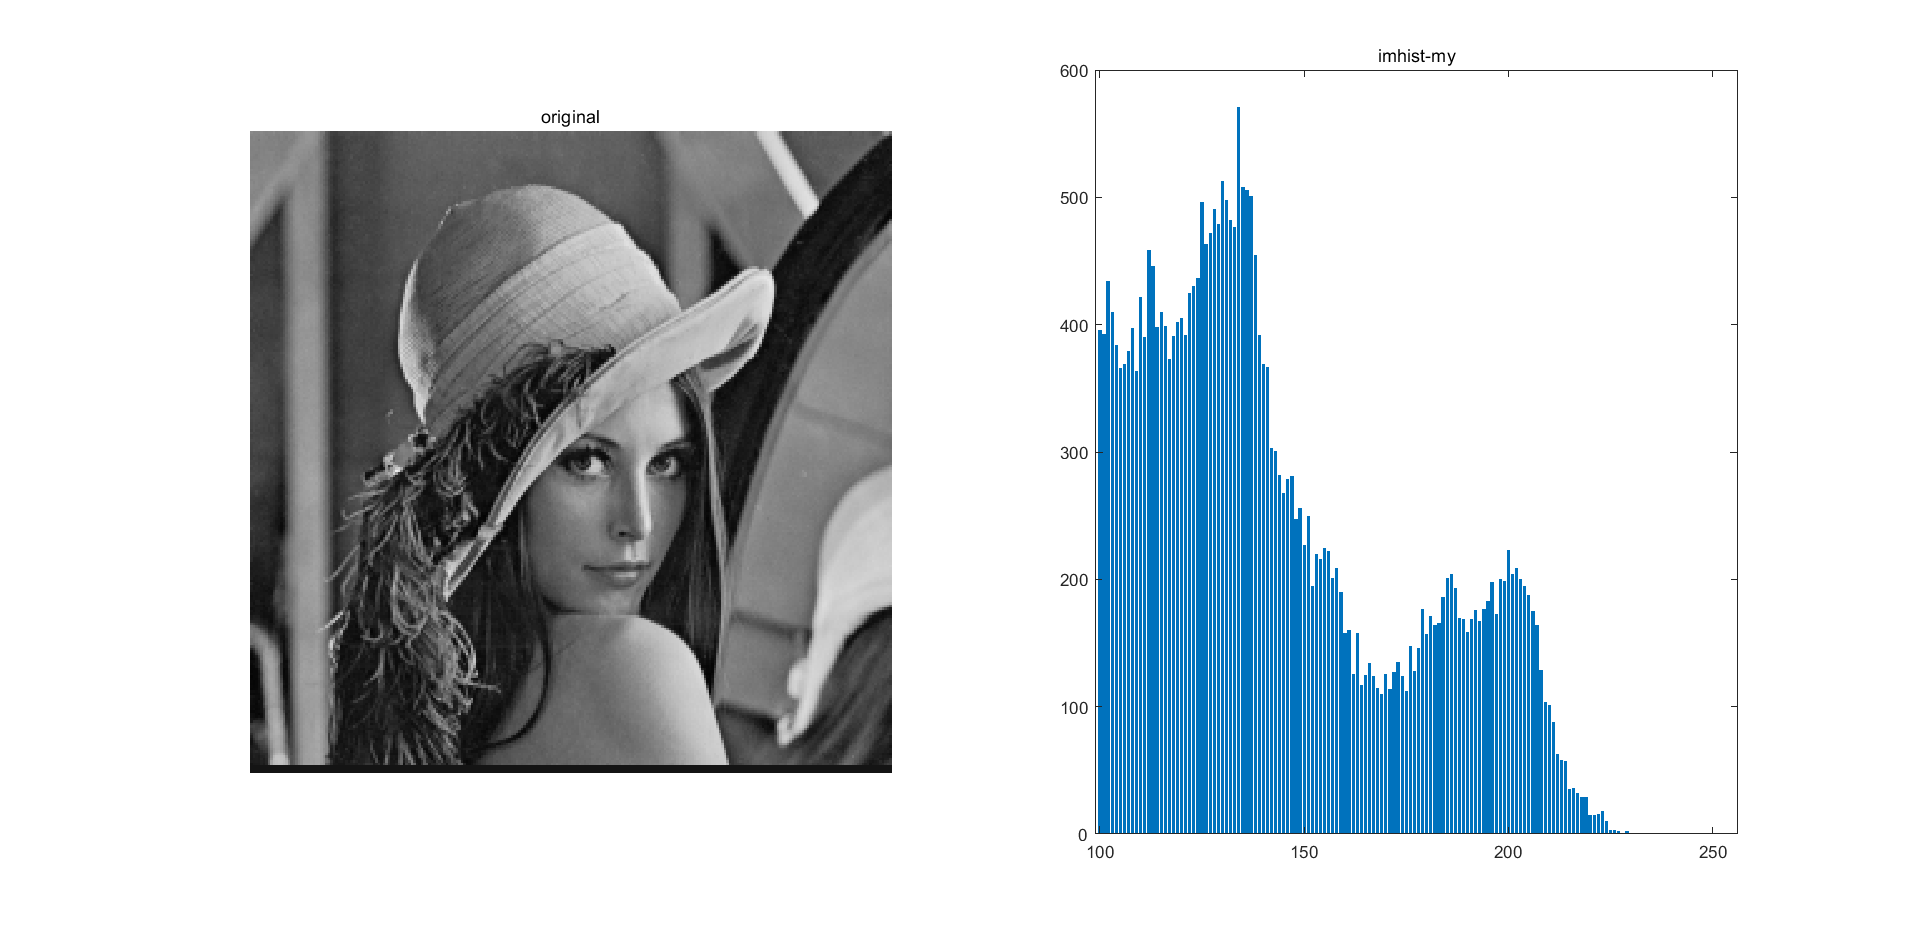
\includegraphics[scale=0.2]{2_3.png}
    \caption{灰度直方图}
\end{figure}
\subsection{\hei 直方图均衡}
\subsubsection{\hei 实验原理}
\begin{enumerate}
    \item 统计图像中各灰度级像素个数 $n_{k}$;
    \item 计算直方图: $\quad p_{r}\left(r_{k}\right)=\frac{n_{k}}{n}$;
    \item 计算累计直方图: $s_{k}=T\left(r_{k}\right)=\sum_{j=0}^{k} p_{r}\left(r_{j}\right)=\sum_{j=0}^{k} \frac{n_{j}}{n}$;
    \item 取整 $\mathrm{S}_{\mathrm{k}}=\operatorname{int}\left[(\mathrm{L}-1) \mathrm{s}_{\mathrm{k}}+\mathrm{0 . 5}\right.$;
    \item 确定映射对应关系: $\mathrm{k} \rightarrow \mathrm{S}_{\mathrm{k}}$;
    \item 对图像进行增强变换 $\left(\mathrm{k} \rightarrow \mathrm{S}_{\mathrm{k}}\right)$。\par
          其中L是灰度等级, $\mathrm{n}$ 是图像总像素数。
\end{enumerate}
\subsubsection{\hei 实验内容}
\begin{enumerate}
    \item 显示一幅图像 pout. bmp 的直方图;
    \item 用直方图均衡对图像 pout. bmp 进行增强;
    \item 显示增强后的图像及其直方图;
    \item 用原始图像 pout.bmp 进行直方图规定化处理,将直方图规定化为高斯分布;
    \item 显示规定化后的图像及其直方图。
\end{enumerate}
\par 得到的结果为:
\begin{figure}[H]
    \centering
    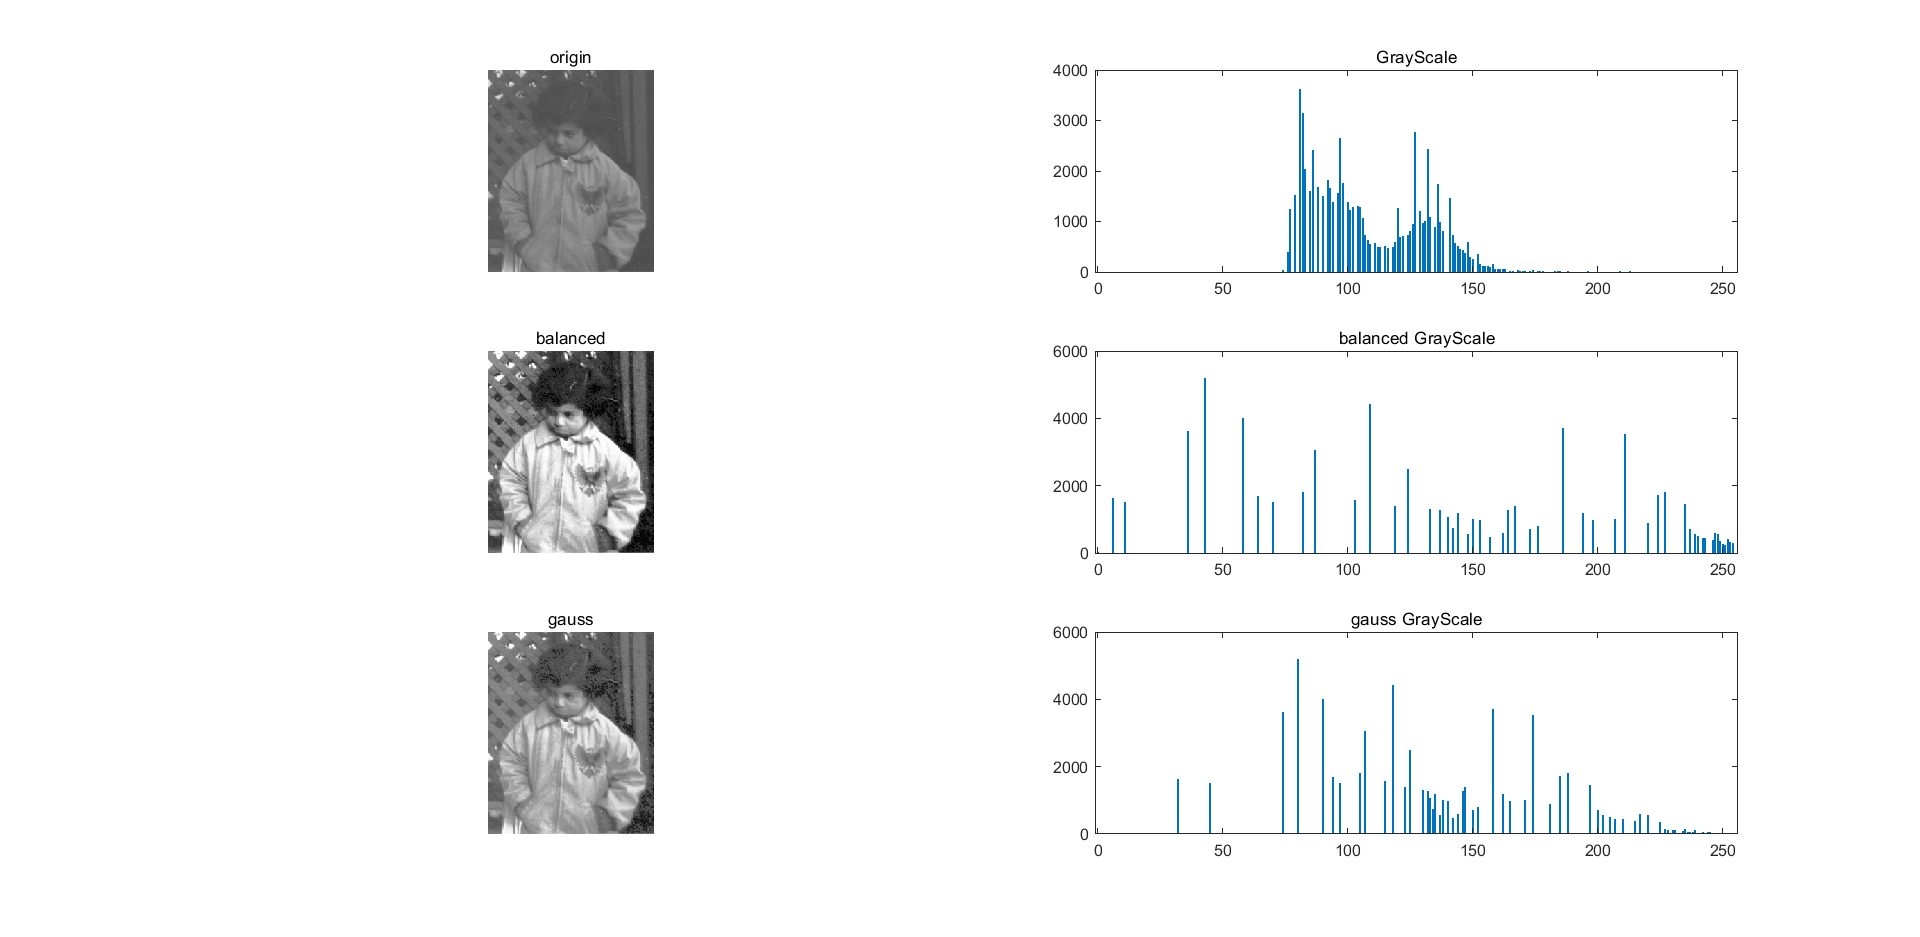
\includegraphics[scale=0.3]{2_4.png}
    \caption{直方图均衡}
\end{figure}
\section{\hei 实验三\ 图像空间域滤波增强}
\subsection{\hei 邻域平均法}
\subsubsection{\hei 实验原理}
用均值滤波器去除图像中的噪声(选 $3 \times 3$ 窗口)
$$
    f\left(x_{0}, y_{0}\right)=\frac{1}{N \times N} \sum f(x, y)
$$
\subsubsection{\hei 实验内容}
用原始图像 lena.bmp 或 cameraman.bmp 分别加产生的 3\%椒盐噪声、高斯噪声、随机
噪声合成有噪声的图像并显示以及邻域平均法去噪后的结果。
\par 得到的结果为:
\begin{figure}[H]
    \centering
    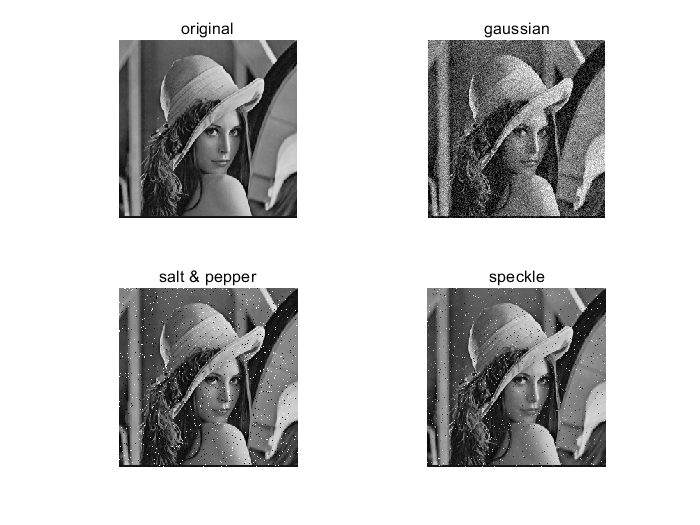
\includegraphics[scale=0.35]{zs.png}
    \caption{有噪声的图像}
\end{figure}
\begin{figure}[H]
    \centering
    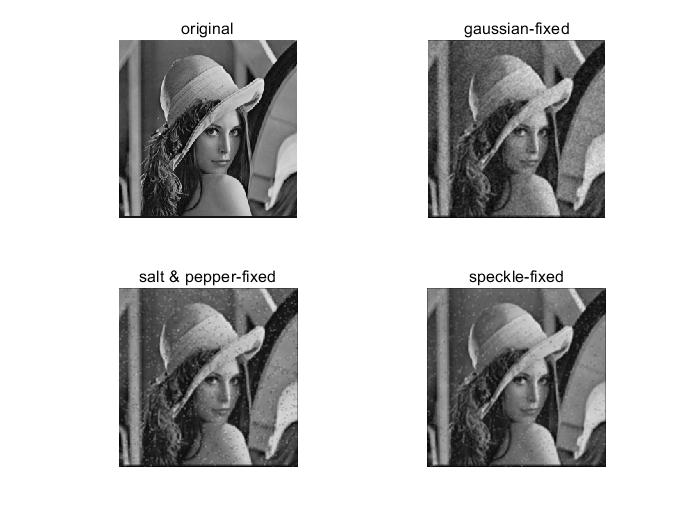
\includegraphics[scale=0.35]{3_1.png}
    \caption{邻域平均法}
\end{figure}
\subsection{\hei 超限邻域平均法}
\subsubsection{\hei 实验原理}
用超限邻域平均法去除图像中的噪声:如果某个像素的灰度值大于其邻域像素的
平均值,且达到了一定水平,则判断该像素为噪声,继而用邻域像素的均值取代这
一像素值,
$$
    g(i, j)=\left\{\begin{array}{ll}
        \frac{1}{N \times N} \sum_{(x, y) \in A} f(x, y), & \left|f(i, j)-\frac{1}{N \times N} \sum_{(x, y) \in A} f(x, y)\right|>T \\
        f(i, j),                                          & \text { 其它 }
    \end{array}\right.
$$
$\mathrm{T}$ 为某一阈值。
\subsubsection{\hei 实验内容}
用原始图像 lena.bmp 或 cameraman.bmp 分别加产生的 3\%椒盐噪声、高斯噪声、随机
噪声合成有噪声的图像并显示以及超限邻域平均法去噪后的结果。
\par 设置阈值为50,得到的结果为:
\begin{figure}[H]
    \centering
    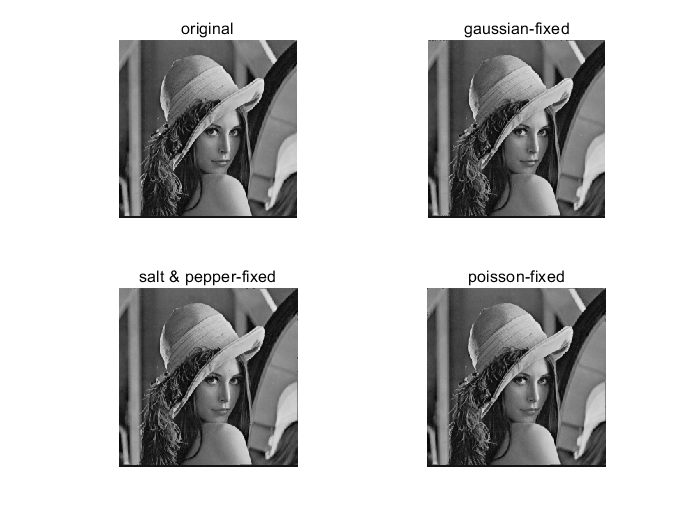
\includegraphics[scale=0.35]{3_2.png}
    \caption{超限邻域平均法}
\end{figure}
\subsection{\hei 中值滤波器}
\subsubsection{\hei 实验原理}
用中值滤波器去除图像中的噪声(选 3x3 窗口做中值滤波);
$$f\left(x_{0}, y_{0}\right)=\operatorname{Med}\left\{f(x, y) \mid x \in\left[x_{0}-N, x_{0}+N\right], y \in\left[y_{0}-N, y_{0}+N\right]\right\}$$
\subsubsection{\hei 实验内容}
用原始图像 lena.bmp 或 cameraman.bmp 分别加产生的 3\%椒盐噪声、高斯噪声、随机
噪声合成有噪声的图像并显示以及中值滤波器去噪后的结果。
\par 得到的结果为:
\begin{figure}[H]
    \centering
    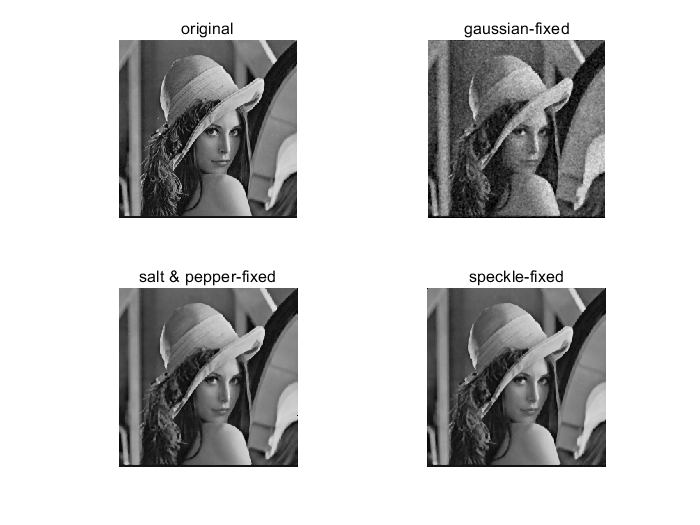
\includegraphics[scale=0.35]{3_3.png}
    \caption{中值滤波器}
\end{figure}
\subsection{\hei 超限中值滤波器}
\subsubsection{\hei 实验原理}
用超限中值滤波器去除图像中的噪声:当某个像素的灰度值超过窗口中像素灰度
值排序中间的那个值,且达到一定水平时,则判断该点为噪声,用灰度值排序中间
的那个值来代替;否则还是保持原来的灰度值。
\subsubsection{\hei 实验内容}
用原始图像 lena.bmp 或 cameraman.bmp 分别加产生的 3\%椒盐噪声、高斯噪声、随机
噪声合成有噪声的图像并显示以及超限中值滤波器去噪后的结果。
\par 设置阈值为50,得到的结果为:
\begin{figure}[H]
    \centering
    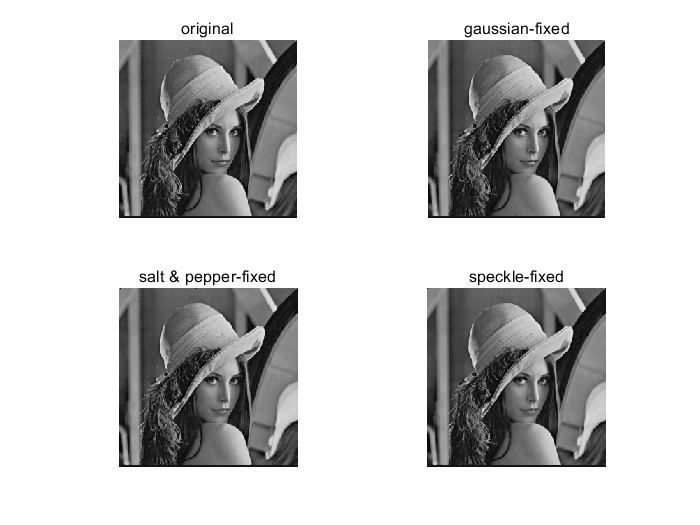
\includegraphics[scale=0.35]{3_4.png}
    \caption{超限中值滤波器}
\end{figure}
\subsection{\hei 分析比较}
\subsubsection{\hei 实验内容}
将四种处理方法的结果与原图比较,注意不同处理方法对边缘的影响。
\par 根据实验结果,可以看出,邻域平均法虽然可以平滑噪声,但使得图像变得模糊,尤其是边缘变得不清晰。超限邻域平均法则效果较好,
在灰度较为连续的区域没有出现模糊的情况,边缘也得到较好的处理,去除噪声的效果更明显。中值滤波器则对高斯噪声的处理效果较差,去除得不够彻底,在处理椒盐噪声和随机噪声时,处理效果好,边缘也没有模糊的情况。
超限中值滤波器,进一步提高了去噪效果,在高斯噪声上也得到了较好的效果,边缘等细节也保留得较好。
\subsection{\hei 边缘检测}
\subsubsection{\hei 实验原理}
边缘检测主要有以下几种常用的算子:
\begin{enumerate}
    \item Roberts 算子 \par 它由下式给出:
          $$
              \boldsymbol{G}[F(\boldsymbol{x}, \boldsymbol{y})] \approx|F(\boldsymbol{x}, \boldsymbol{y})-F(\boldsymbol{x}+1, \boldsymbol{y}+1)|+|F(\boldsymbol{x}+1, \boldsymbol{y})-F(\boldsymbol{x}, \boldsymbol{y}+1)|
          $$
          其中 F(x,y)是具有整数像素坐标的输入图像。
    \item Sobel 算子 \par
          图像中的每个点都用下面的两个模板做卷积,一个对通常的垂直边缘响应最大,另一 个对水平边缘响应最大,两个卷积的最大值作为该点的输出位。 $$\begin{tabular}{|l|l|l|}
              \hline$-1$ & $-2$ & $-1$ \\
              \hline 0   & 0    & 0    \\
              \hline 1   & 2    & 1    \\
              \hline
          \end{tabular}$$$$ \begin{tabular}{|l|l|l|}
              \hline$-1$ & 0 & 1 \\
              \hline$-2$ & 0 & 2 \\
              \hline$-1$ & 0 & 1 \\
              \hline
          \end{tabular}$$
    \item Prewitt 算子 \par 下面的两个模板形成了 Prewitt 算子,和使用 Sobel 算子的方法一样。 $$\begin{tabular}{|l|l|l|}
                  \hline$-1$ & $-1$ & $-1$ \\
                  \hline 0   & 0    & 0    \\
                  \hline 1   & 1    & 1    \\
                  \hline
              \end{tabular} $$$$\begin{tabular}{|l|l|l|}
                  \hline 1 & 0 & $-1$ \\
                  \hline 1 & 0 & $-1$ \\
                  \hline 1 & 0 & $-1$ \\
                  \hline
              \end{tabular}$$
    \item 拉普拉斯算子
          $$
              \nabla^{2} f=\frac{\partial^{2} f}{\partial x^{2}}+\frac{\partial^{2} f}{\partial y^{2}}=f(i-1, j)+f(i+1, j)+f(i, j+1)+f(i, j-1)-4 f(i, j)
          $$
          分别用模板:
          $$\left[\begin{array}{ccc}0 & 1 & 0 \\ 1 & -4 & 1 \\ 0 & 1 & 0\end{array}\right]$$ 和 $$\left[\begin{array}{ccc}-1 & -1 & -1 \\ -1 & 8 & -1 \\ -1 & -1 & -1\end{array}\right]$$ 进行边缘检测
          (用拉普拉斯算子:将输出图灰度值范围通过尺度变换变回到:0-255 范围; )
    \item Canny 算子
          \begin{enumerate}
              \item 用高斯滤波器平滑图像;
              \item  用一阶偏导的有限差分来计算梯度的幅值和方向;
              \item  对梯度幅值进行非极大值抑制;
              \item  用双间值算法检测和连接边缘。
          \end{enumerate}
\end{enumerate}
\subsubsection{\hei 实验内容}
要求对 blood.bmp、 lena.bmp,分别用前面所述的算子进行边缘检测,显示边缘
检测结果图像。
\par 得到的结果为:
\begin{figure}[H]
    \centering
    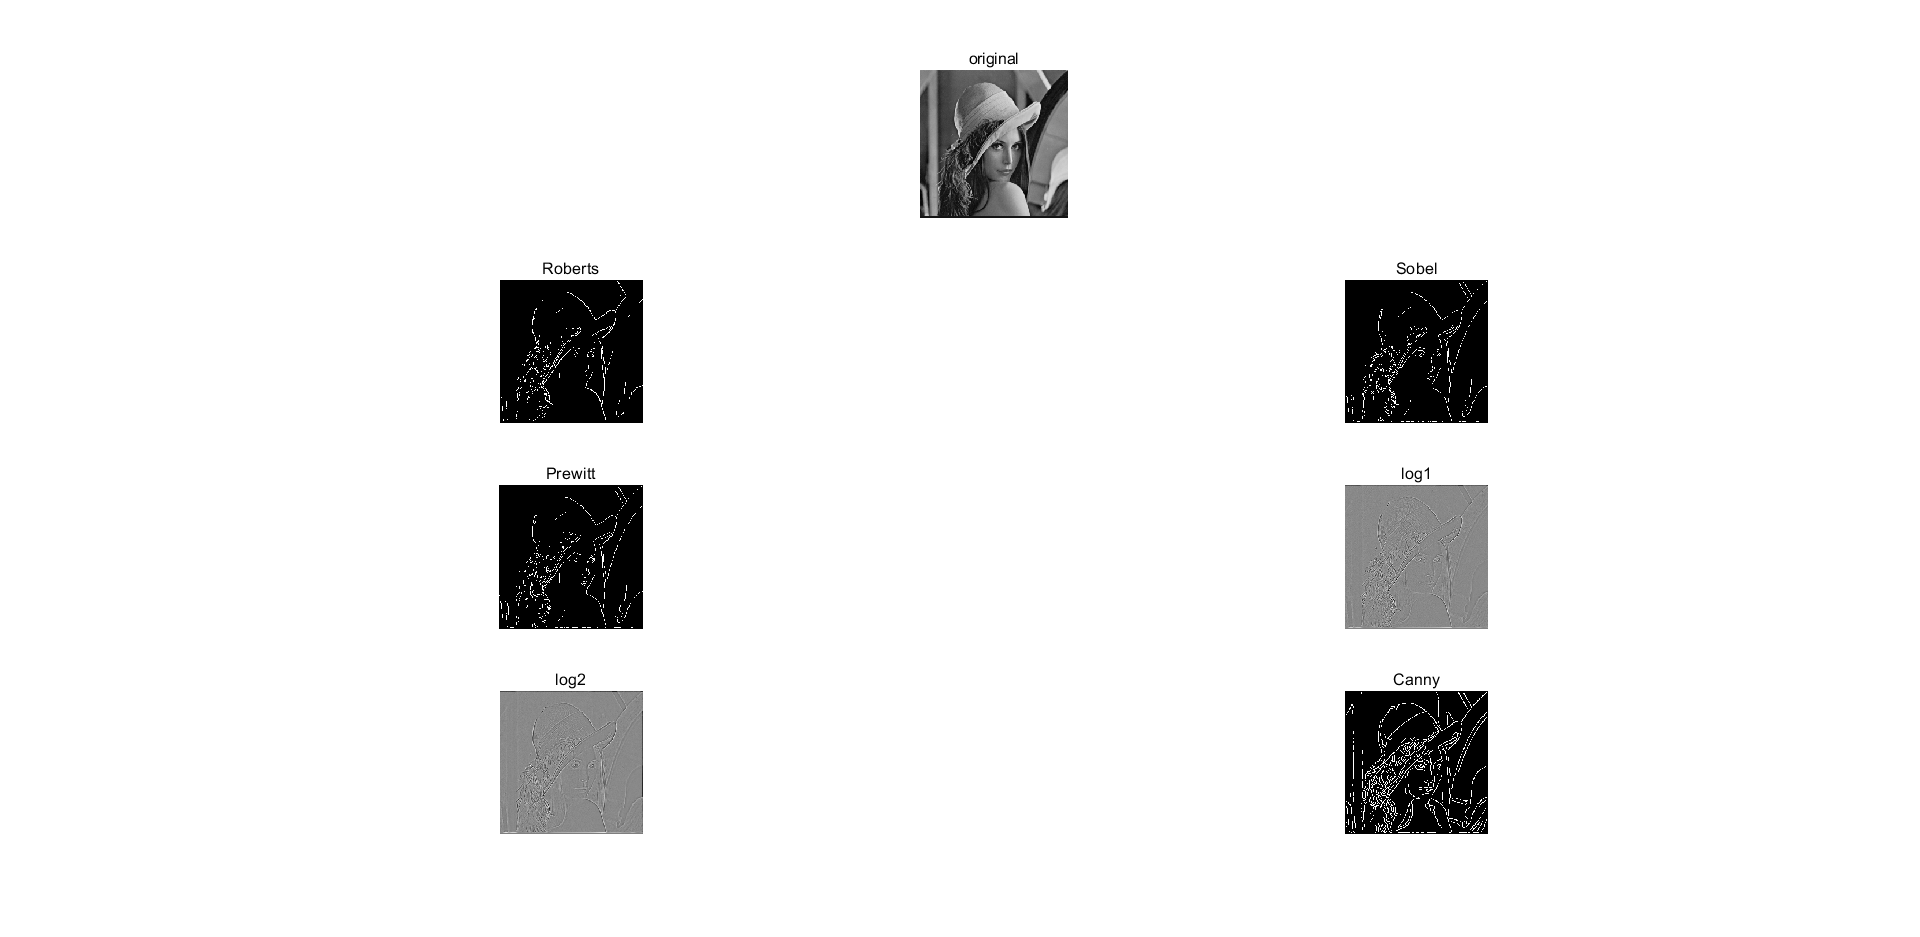
\includegraphics[scale=0.35]{lena.png}
    \caption{边缘检测(lena.bmp)}
\end{figure}
\par 得到的结果为:
\begin{figure}[H]
    \centering
    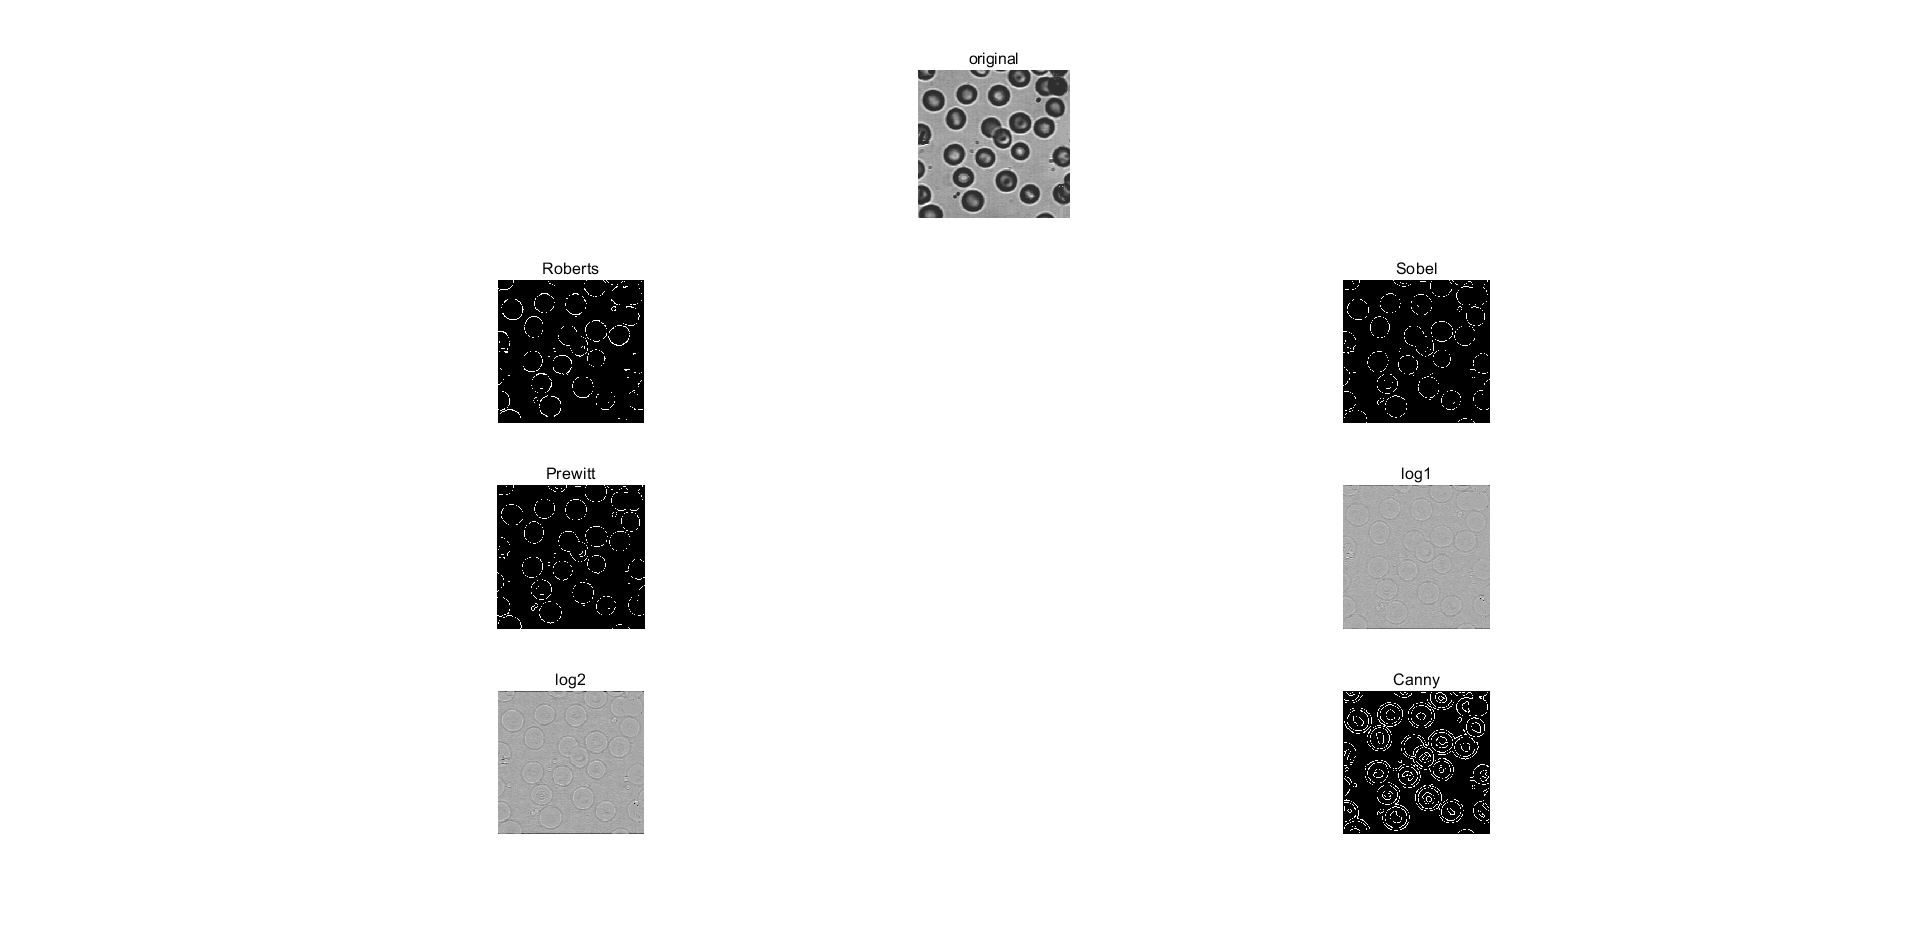
\includegraphics[scale=0.35]{blood.png}
    \caption{边缘检测(blood.bmp)}
\end{figure}
\section{\hei 实验四\ 图像变换及频域滤波增强}
\subsection{\hei Fourier 变换}


\subsubsection{\hei 实验内容}
用 Fourier 变换算法,对 rect1.bmp 和 rect2.bmp 图像作二维 Fourier 变换;并显示
其频谱。要求对幅度作变换(由于高、低频幅度相差很大),将低频移到中心点。
\par 得到的结果为:
\begin{figure}[H]
    \centering
    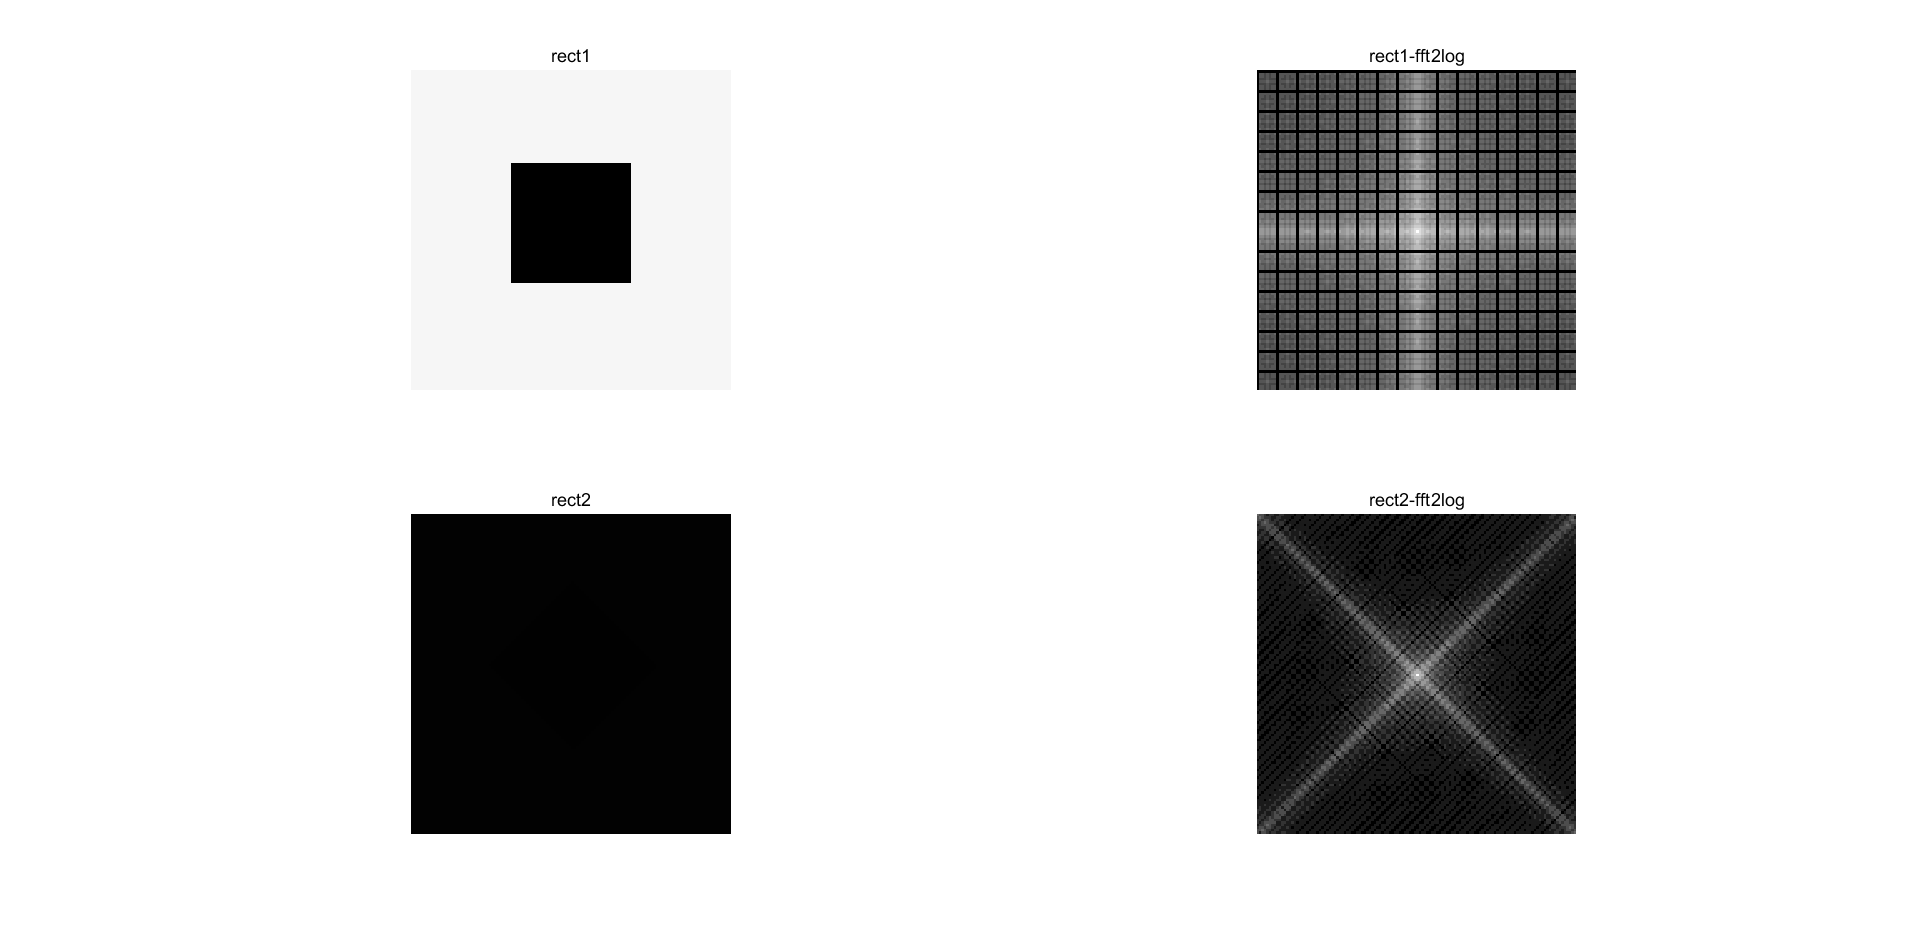
\includegraphics[scale=0.35]{4_1.png}
    \caption{Fourier 变换1}
\end{figure}
用 Fourier 系数的幅度进行 Fourier 反变换,并显示其图像;用 Fourier 系数的相位
进行 Fourier 反变换,并显示其图像;比较 3、4 的结果,
评价人眼对图像幅频特性和相频特性的敏感度。将图像的 Fourier 变换置为其共轭后进行
反变换,显示其图像,并与原始图像比
较其差异。
\par 得到的结果为:
\begin{figure}[H]
    \centering
    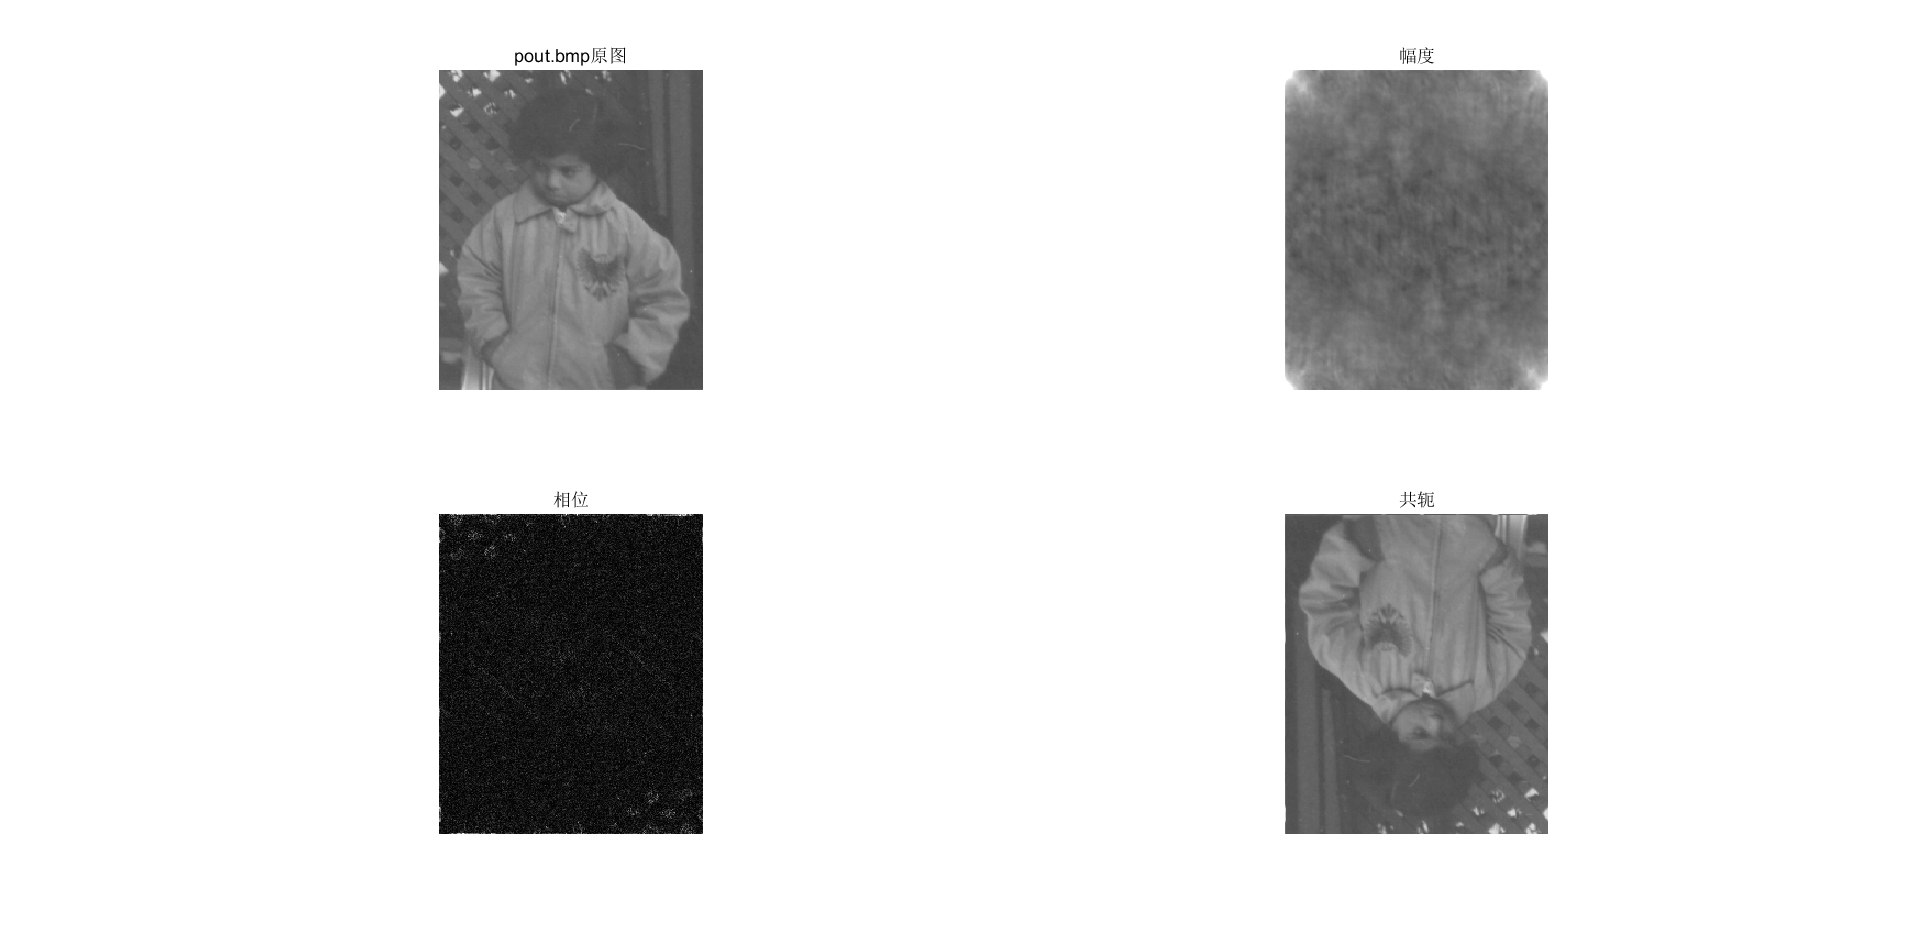
\includegraphics[scale=0.35]{4_2-4.png}
    \caption{Fourier 变换2}
\end{figure}
\par 可以看出人眼对图像的幅频特性较为敏感,对相频特性则较不敏感。在该例子中,图像的 Fourier 变换共轭后再进行逆变换得到的图像为原图旋转$180^o$的结果。
\subsection{\hei 低通滤波器}

\subsubsection{\hei 实验内容}
对图像 pout.bmp、Girl.bmp 分别采用理想低通滤波器、巴特沃斯低通滤波器和高
斯低通滤波器(截止频率自选),再做反变换,观察不同截止频率下采用不同低通
滤波器得到的图像与原图像的区别,特别注意振铃效应。
\par 选择d=30,得到的结果为:
\begin{figure}[H]
    \centering
    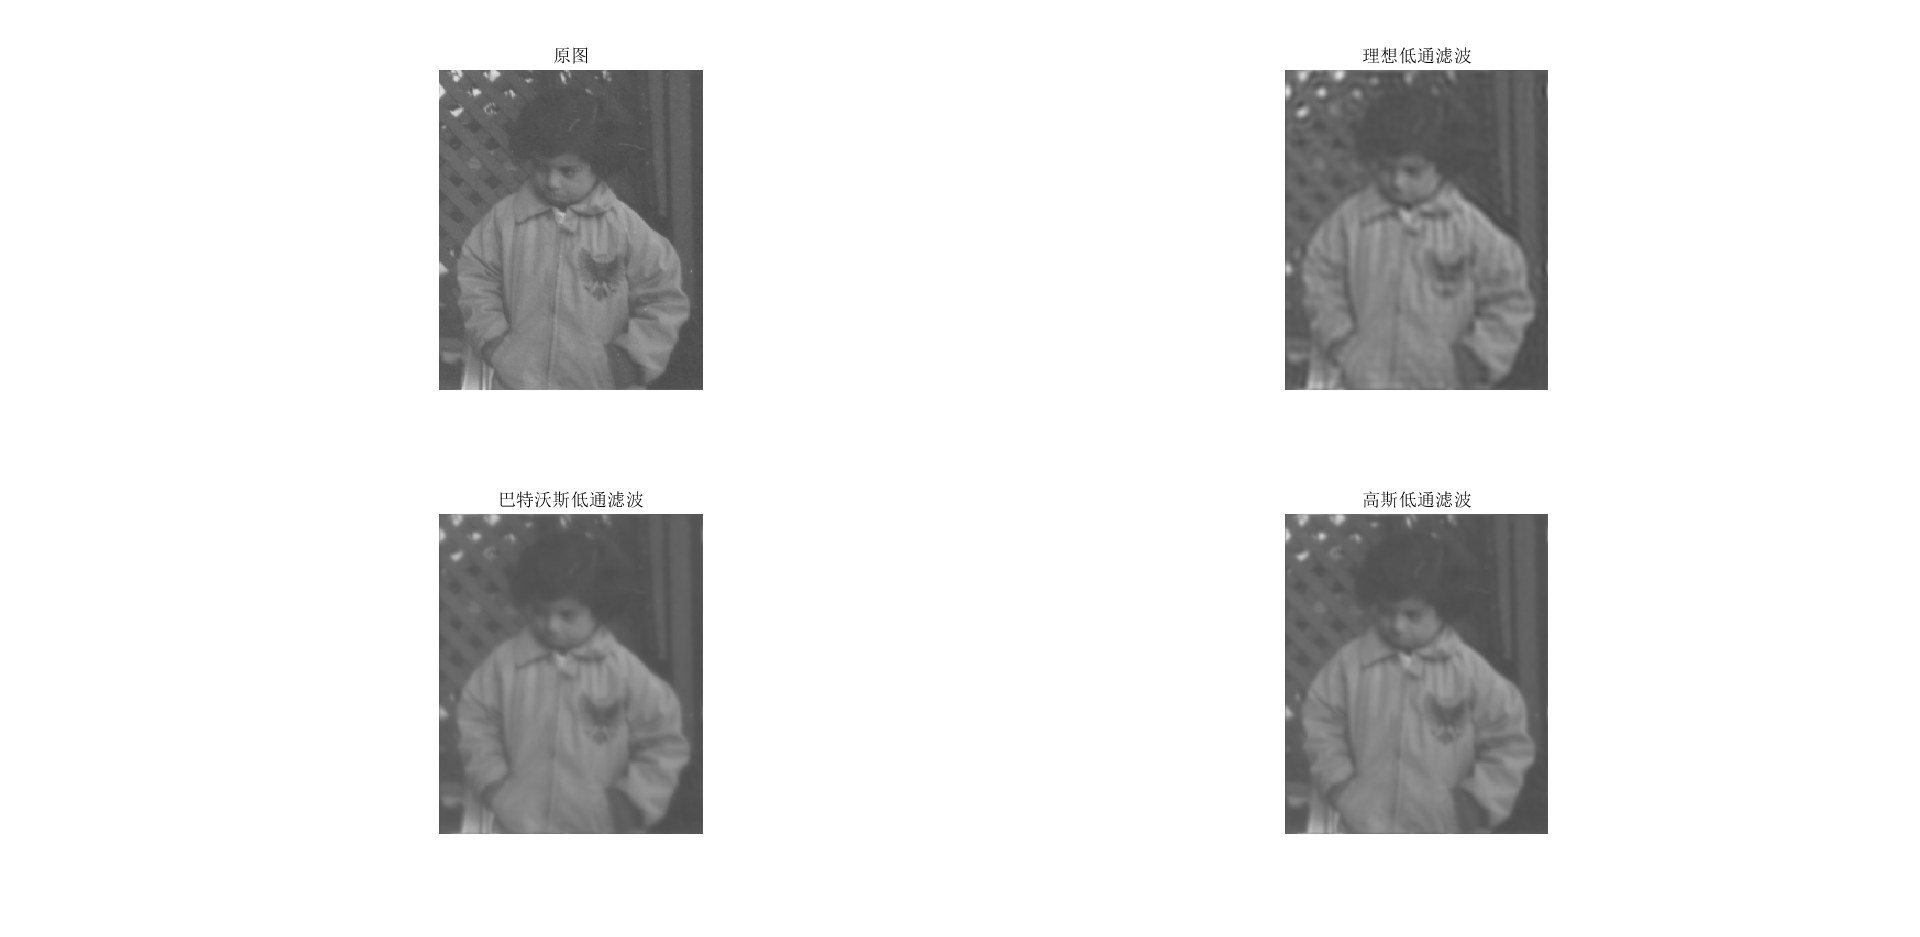
\includegraphics[scale=0.35]{4_5_1.png}
    \caption{低通滤波器(pout.bmp)}
\end{figure}
\par 选择d=30,得到的结果为:
\begin{figure}[H]
    \centering
    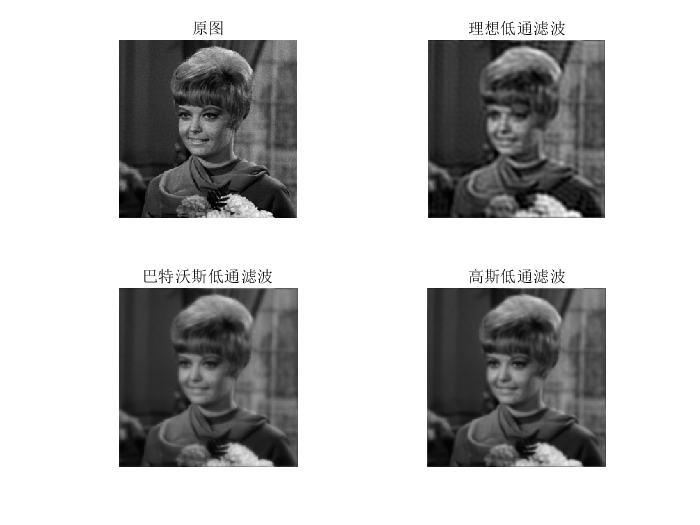
\includegraphics[scale=0.6]{4_5_2.png}
    \caption{低通滤波器(Girl.bmp)}
\end{figure}
\subsection{\hei 低通滤波器去噪}

\subsubsection{\hei 实验内容}
对原始图像 Girl.bmp 分别加椒盐噪声、高斯噪声,产生有噪声图像,利用上述低
通滤波器进行去噪,对比去噪效果。
\par 选择d=30,得到的结果为:
\begin{figure}[H]
    \centering
    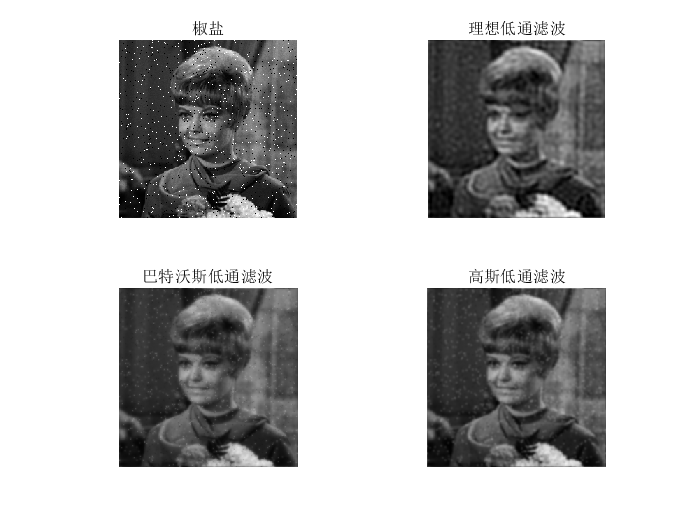
\includegraphics[scale=0.6]{4_6_1.png}
    \caption{低通滤波器去噪(椒盐噪声)}
\end{figure}
\par 选择d=30,得到的结果为:
\begin{figure}[H]
    \centering
    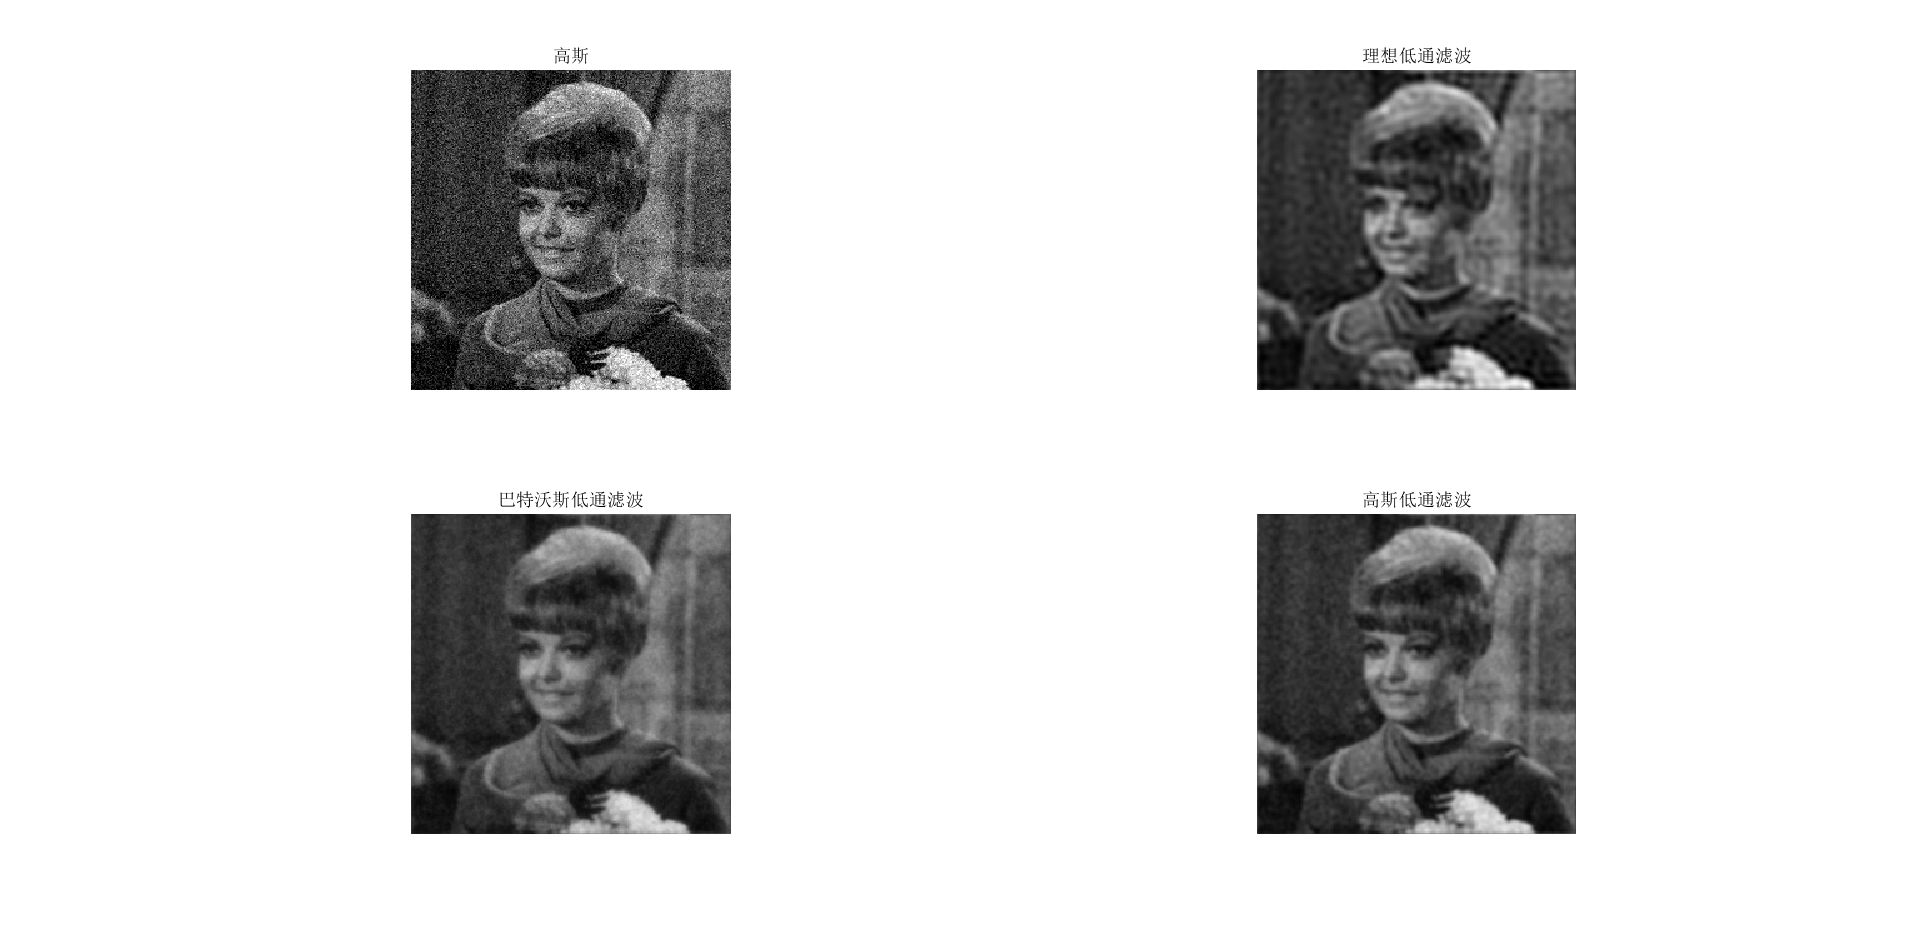
\includegraphics[scale=0.3]{4_6_2.png}
    \caption{低通滤波器去噪(高斯噪声)}
\end{figure}

\subsection{\hei 高通滤波器}
对图像 pout.bmp、Girl.bmp 分别采用高通滤波器、巴特沃斯高通滤波器和高斯高
通滤波器(截止频率自选),再做反变换,观察不同截止频率下采用不同高通滤波
器得到的图像与原图像的区别,特别注意振铃效应。
\par 选择d=5,得到的结果为:
\begin{figure}[H]
    \centering
    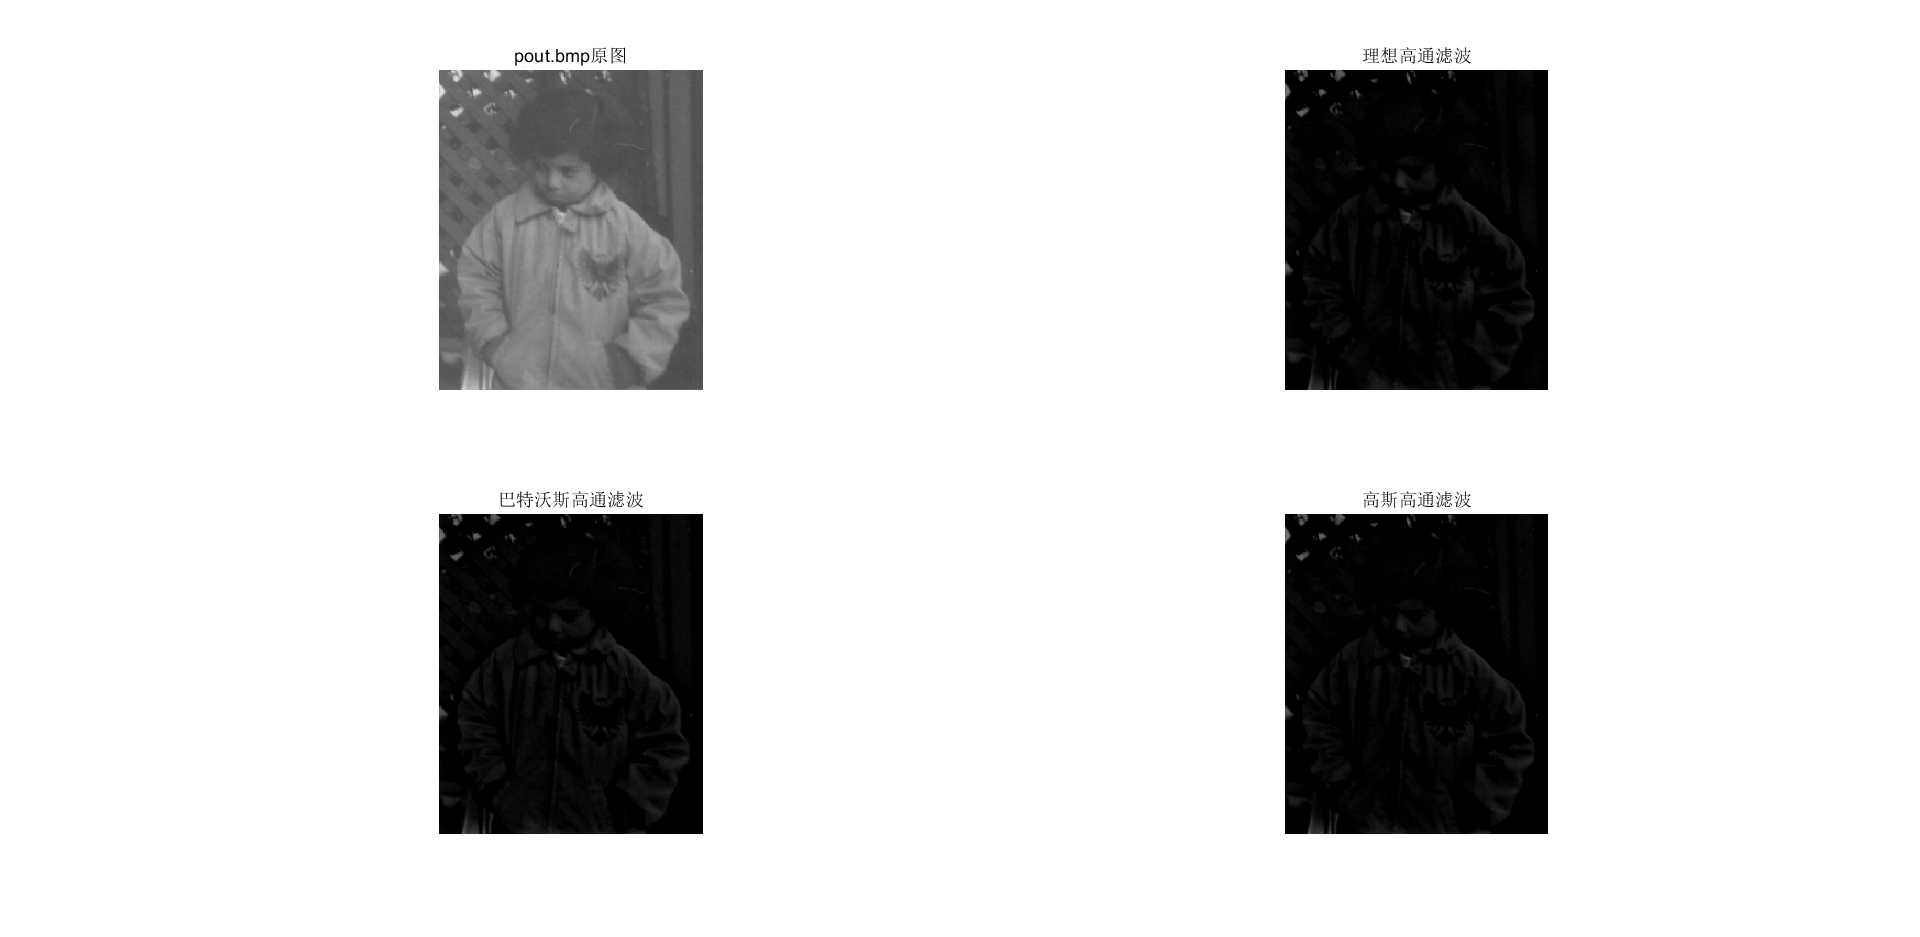
\includegraphics[scale=0.35]{4_7_1.png}
    \caption{高通滤波器(pout.bmp)}
\end{figure}
\par 选择d=5,得到的结果为:
\begin{figure}[H]
    \centering
    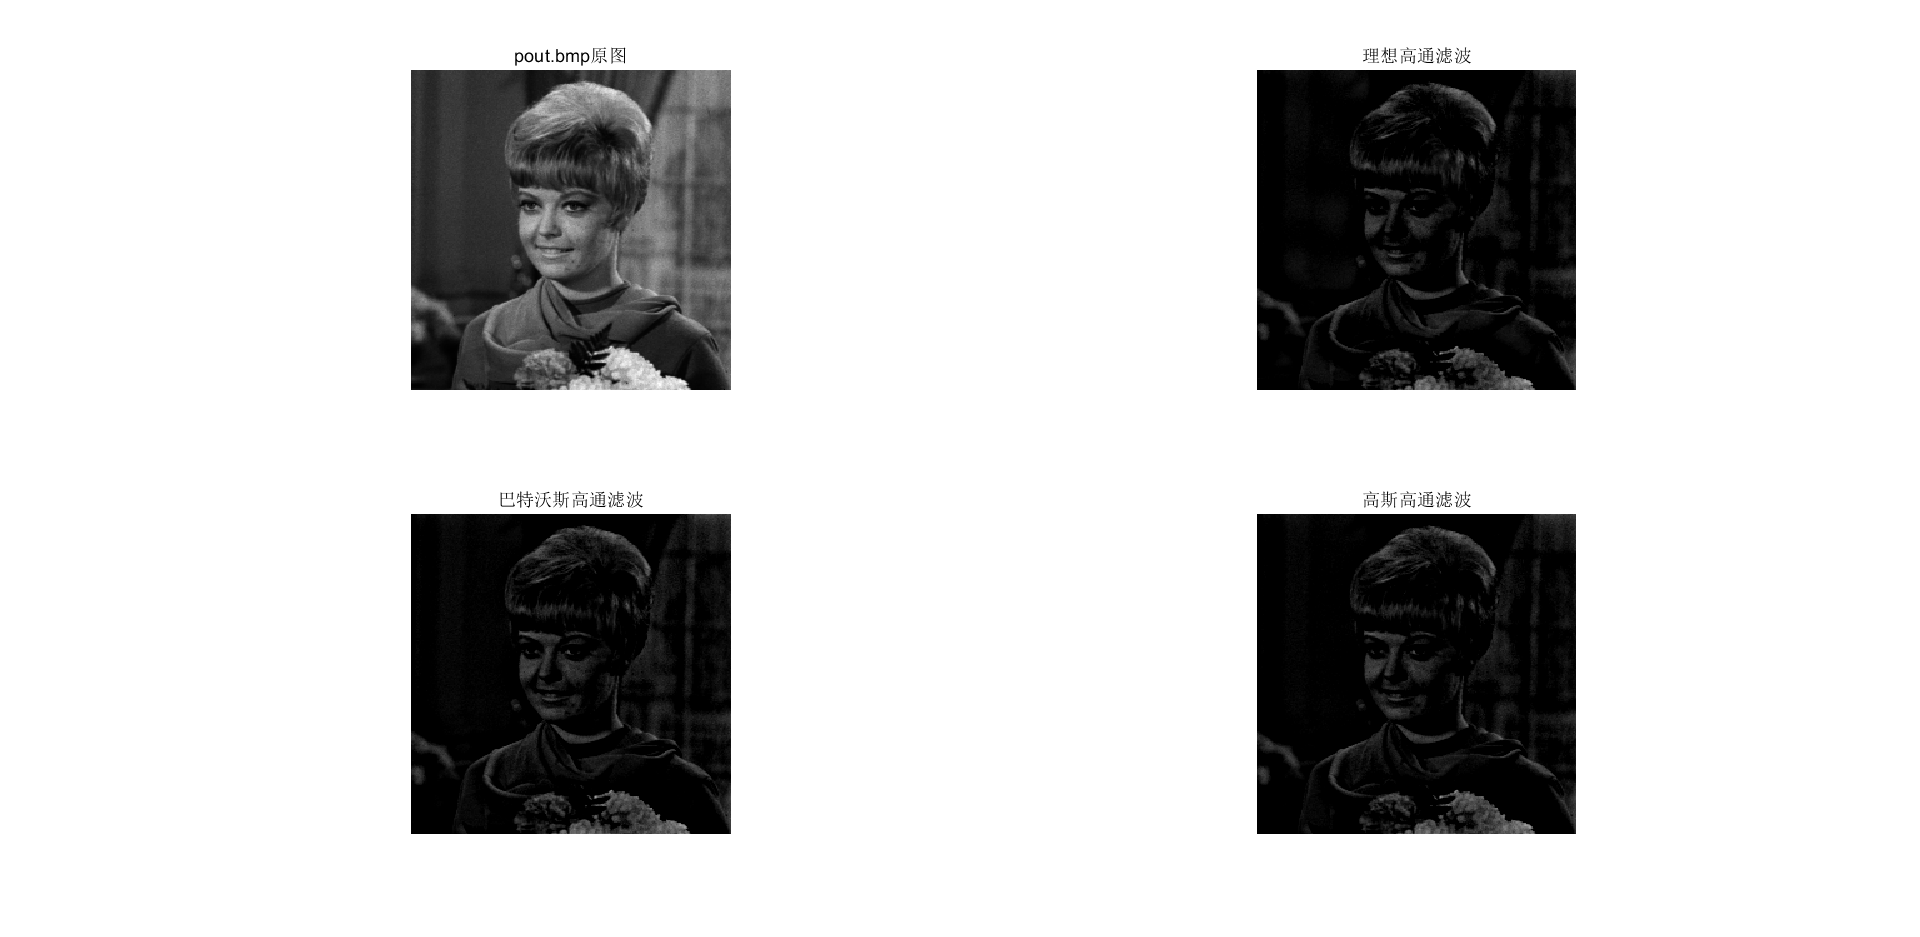
\includegraphics[scale=0.35]{4_7_2.png}
    \caption{高通滤波器(Girl.bmp)}
\end{figure}
\subsection{\hei 低通滤波器去噪}

\subsubsection{\hei 高频增强滤波}
对图像 pout.bmp 经过高频增强滤波,再进行直方图均衡化,显示结果图像; 对
图像 pout.bmp 先进行直方图均衡化,再经过高频增强滤波,显示结果图像;观察
对比不同处理顺序对结果图像的影响。
\par 得到的结果为:
\begin{figure}[H]
    \centering
    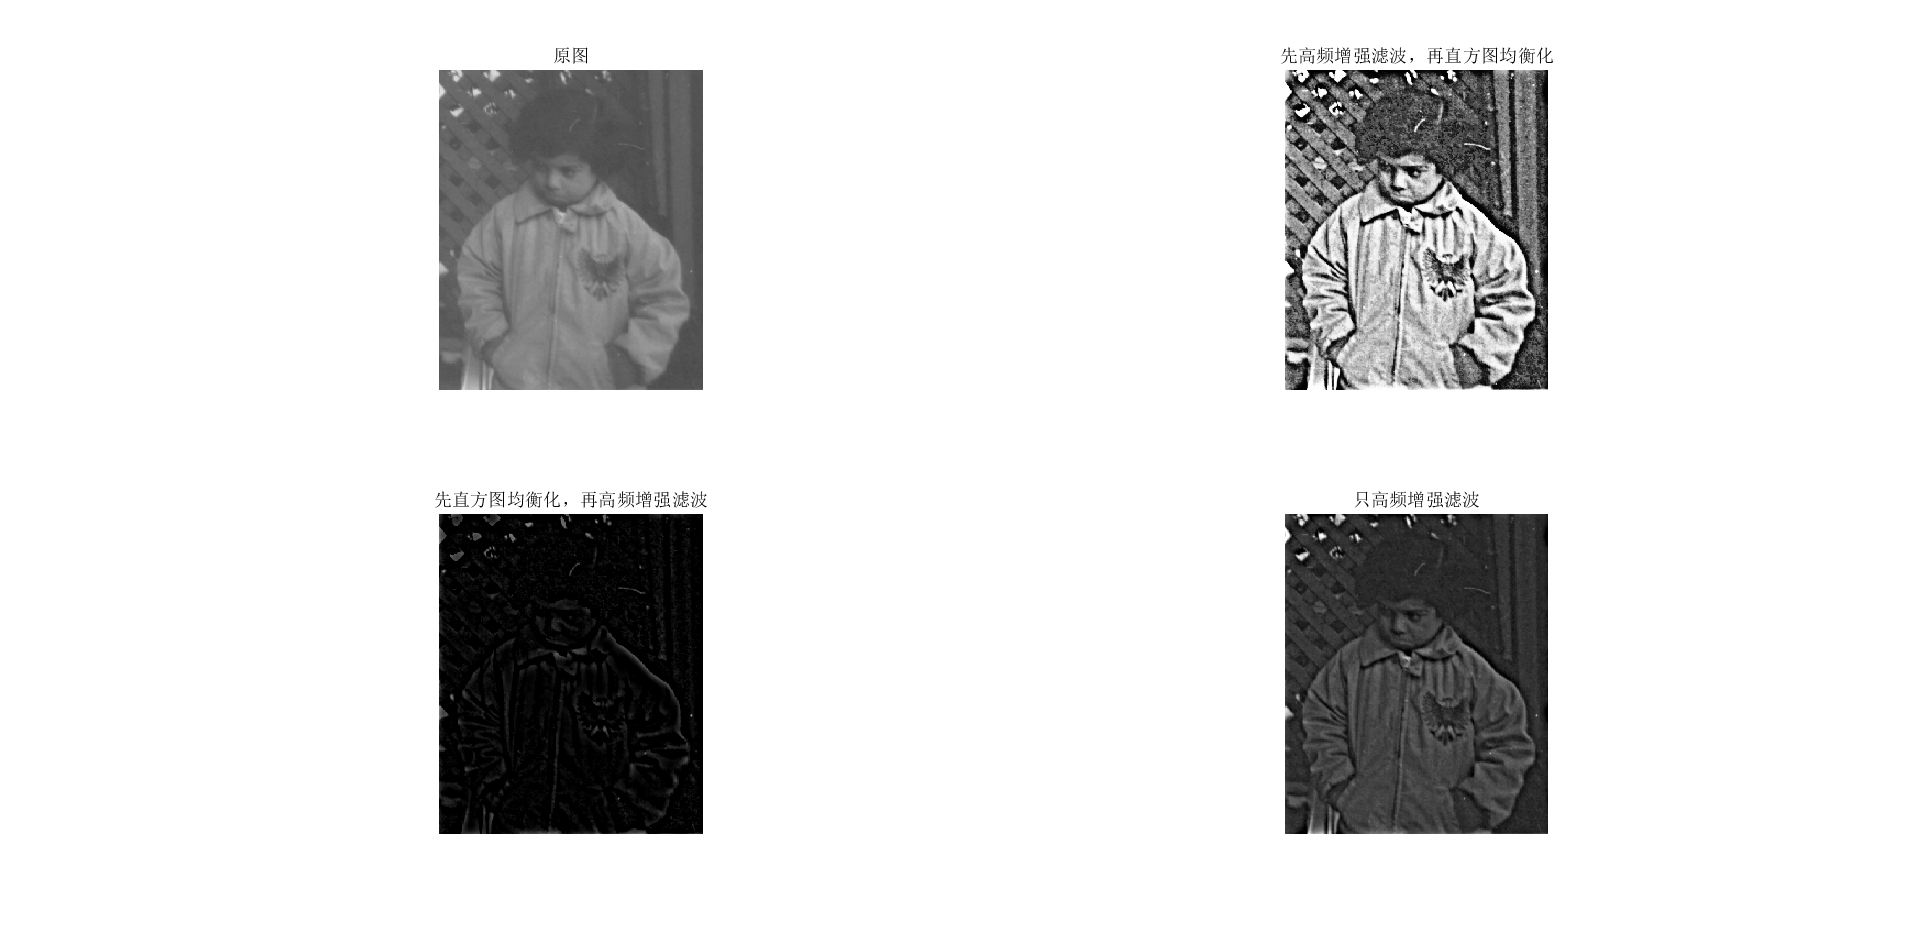
\includegraphics[scale=0.35]{4_8.png}
    \caption{高频增强滤波}
\end{figure}
\section{\hei 实验五\ 图像恢复与图像分割}
\subsection{\hei 逆滤波与维纳滤波}
\subsubsection{\hei 实验内容}
对图像 flower2.jpg 加高斯噪声,产生有噪声图像,分别对其采用逆滤波和维纳滤
波进行恢复,显示、对比分析恢复结果图像。
\par 得到的结果为:
\begin{figure}[H]
    \centering
    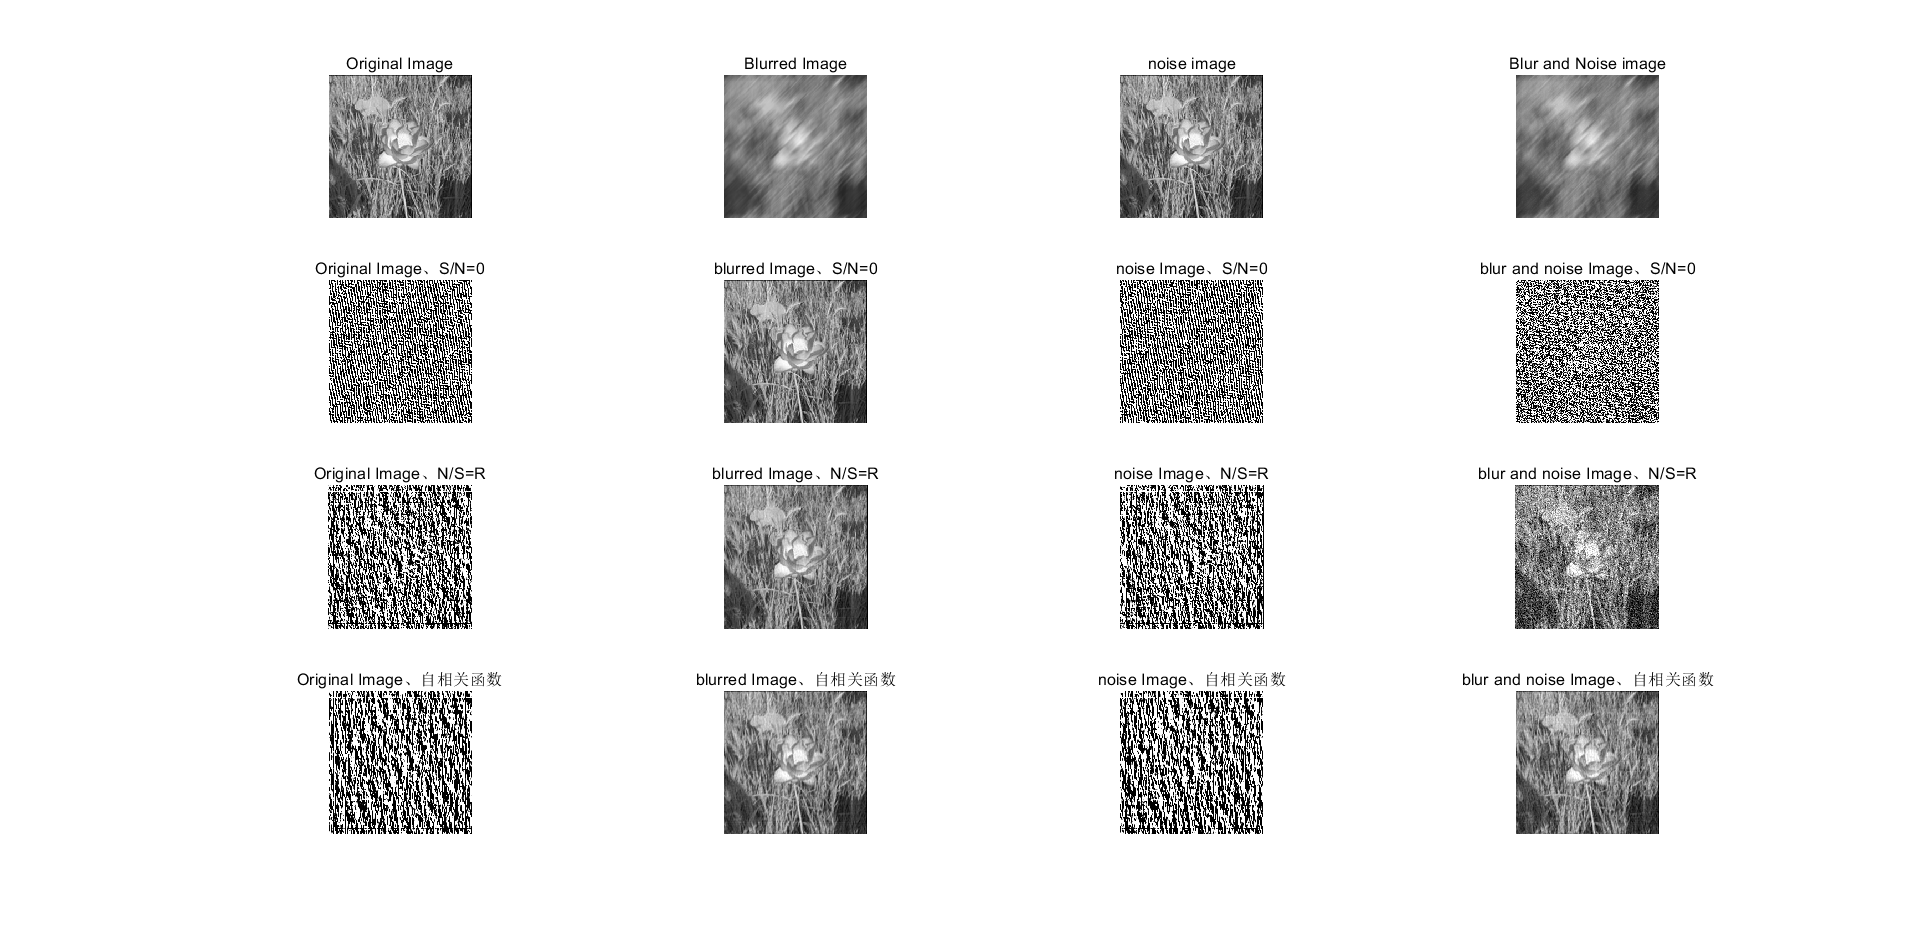
\includegraphics[scale=0.35]{5_1.png}
    \caption{逆滤波与维纳滤波}
\end{figure}
\par 说明:第一列为原图,第二列为运动模糊,第三列为加高斯噪声,第四列为运动模糊加高斯噪声。第一行为滤波前,第二行为逆滤波,第三行为维纳滤波,第四行为使用自相关函数作为参数进行滤波。
\subsection{\hei 大津法}
\subsubsection{\hei 实验原理}
$\mathrm{OTSU}$ 是基于最大类间方差的自适应间值选取法,Matlab 工具箱提供的 graythresh 函数求取间值采用的正是 Ostu 法。 $\mathrm{OTSU}$ 算法步骤如下:
\begin{enumerate}
    \item 统计灰度级中每个像素在整幅图像中的个数。
    \item 计算每个像素在整幅图像的概率分布。
    \item 对灰度级进行遍厂枝索,讲算当前灰度值下前景背景类间概率。
    \item 通过目标函数计算出类内与类间方差下对应的间值。
\end{enumerate} 
对于图像 $\mathrm{I}(\mathrm{x}, \mathrm{y})$, 前景(即目标)和背景的分割间值记作 $\mathrm{T}$, 属于前景的像素点数占整幅
图像的比例记为 $\omega 0$, 其平均灰度 $\mu 0 ;$ 背景像素点数占整幅图像的比例为 $\omega 1$, 其平均
灰度为 $\mu 1$ 。图像的总平均灰度记为 $\mu$ ,类间方差记为 $\mathrm{g}_{\circ}$
假设图像的背景较暗,并且图像的大小为 $\mathrm{M} \times \mathrm{N}$, 图像中像素的灰度值小于间值 $\mathrm{T}$ 的
像素个数记作 $\mathrm{N} 0$ ,像素灰度大于间值 $\mathrm{T}$ 的像素个数记作 $\mathrm{N} 1$, 则有:
$$
\begin{aligned}
&\omega 0=\mathrm{N} 0 / \quad(\mathrm{M} \times \mathrm{N}) \\
&\omega 1=\mathrm{N} 1 / \quad(\mathrm{M} \times \mathrm{N}) \\
&\mathrm{N} 0+\mathrm{N} 1=\mathrm{M} \times \mathrm{N} \\
&\omega 0+\omega 1=1 \\
&\mu=\omega 0^{*} \mu 0+\omega 1^{*} \mu 1 \\
&\mathrm{~g}=\omega 0^{*}(\mu 0-\mu)^{\wedge} 2+\omega 1^{*}(\mu 1-\mu)^{\wedge} 2
\end{aligned}
$$
将式(5)代入式(6),得到等价公式: $\quad \mathrm{g}=\omega 0^{*} \omega 1^{*}(\mu 0-\mu 1)^{\wedge} 2$
采用遍历的方法可以得到类间方差最大的间值 $\mathrm{T}_{\circ}$
\subsubsection{\hei 实验内容}

对图像 lena.bmp 采用大津法(OTSU)自动选取阈值进行分割,显示分割二值化
结果图像。
\par 得到的结果为:
\begin{figure}[H]
    \centering
    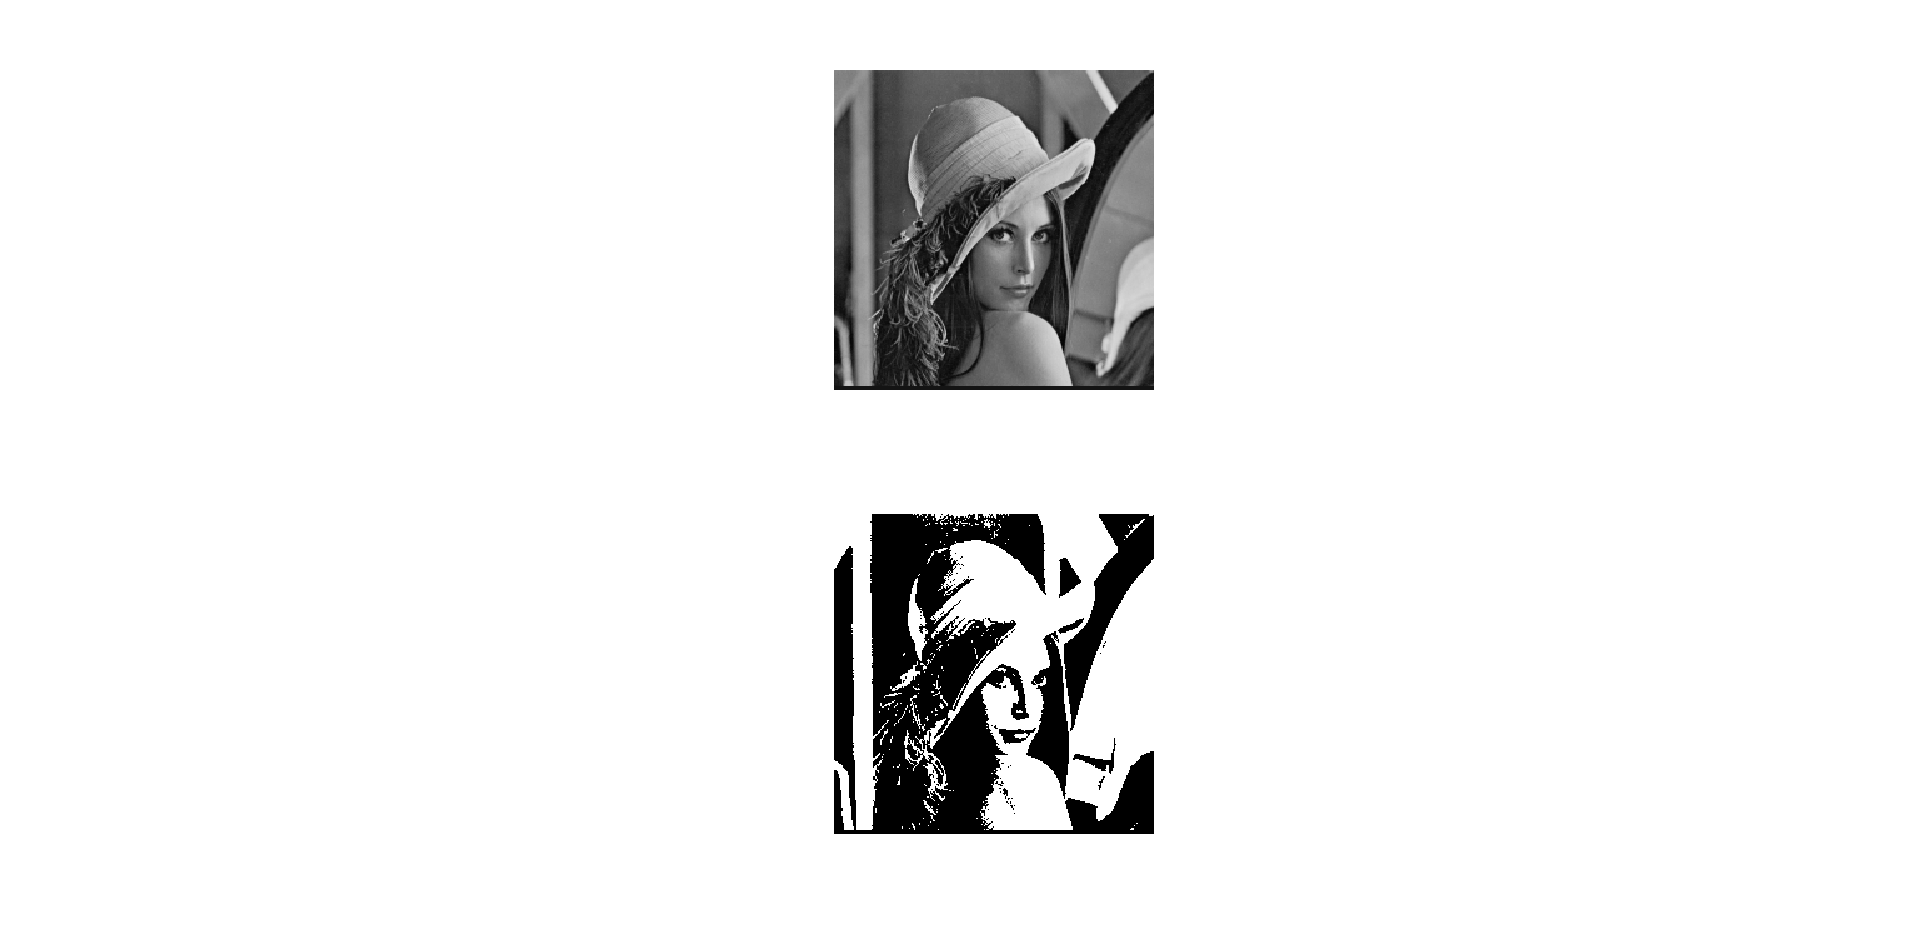
\includegraphics[scale=0.35]{5_2.png}
    \caption{大津法}
\end{figure}
\subsection{\hei 区域分割}
\subsubsection{\hei 实验内容}
对图像 cameraman.bmp 采用四叉树表达的迭代区域分裂合并算法进行分割。显示
分割结果图像。
\par 得到的结果为:
\begin{figure}[H]
    \centering
    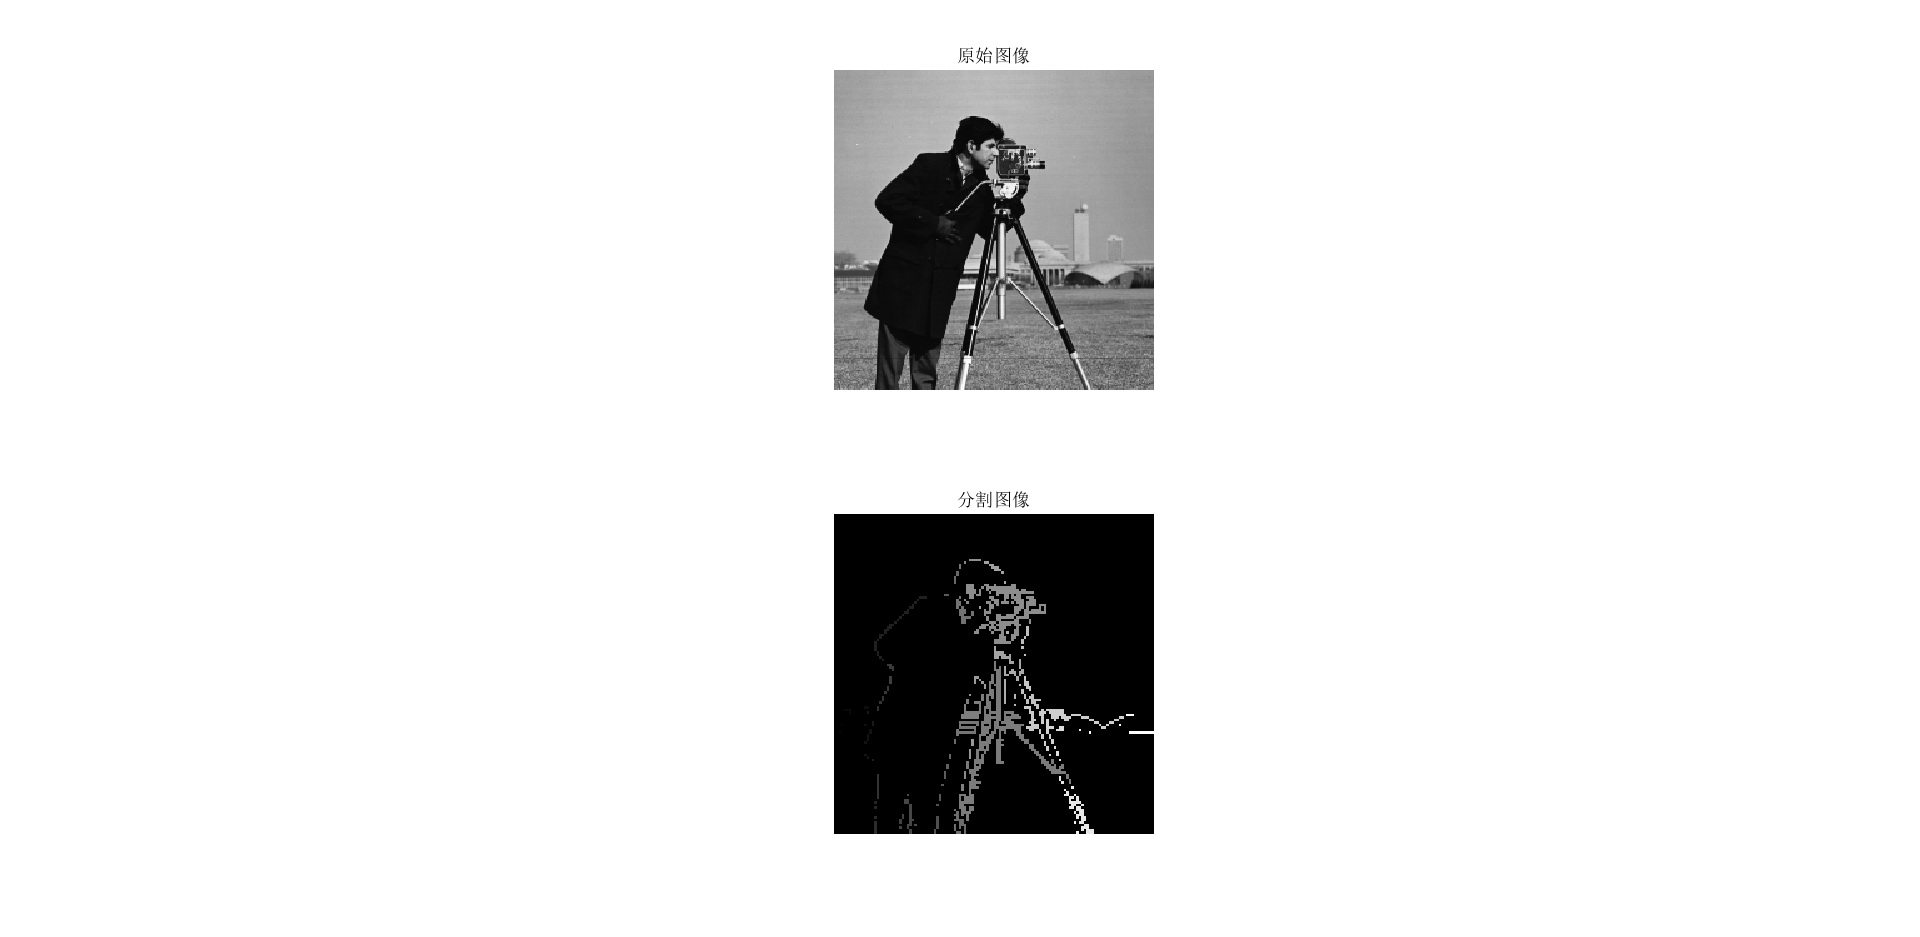
\includegraphics[scale=0.35]{5_3.png}
    \caption{区域分裂合并}
\end{figure}
\end{document}